%%%%%%%% ICML 2025 EXAMPLE LATEX SUBMISSION FILE %%%%%%%%%%%%%%%%%

\documentclass{article}

% Recommended, but optional, packages for figures and better typesetting:
\usepackage{microtype}
\usepackage{graphicx}
% \usepackage{subfigure}
\usepackage{svg}
\usepackage{pgfplots}
\usetikzlibrary{patterns}
\usepackage{booktabs} % for professional tables
\usepackage{subcaption}
\usepackage{longtable}
\usepackage{tablefootnote}

% hyperref makes hyperlinks in the resulting PDF.
% If your build breaks (sometimes temporarily if a hyperlink spans a page)
% please comment out the following usepackage line and replace
% \usepackage{icml2025} with \usepackage[nohyperref]{icml2025} above.
\usepackage{hyperref}


% Attempt to make hyperref and algorithmic work together better:
\newcommand{\theHalgorithm}{\arabic{algorithm}}

% Use the following line for the initial blind version submitted for review:
% \usepackage{icml2025}

% If accepted, instead use the following line for the camera-ready submission:
\usepackage[accepted]{icml2025}

% For theorems and such
\usepackage{amsmath}
\usepackage{amssymb}
\usepackage{mathtools}
\usepackage{amsthm}

% if you use cleveref..
\usepackage[capitalize,noabbrev]{cleveref}

%%%%%%%%%%%%%%%%%%%%%%%%%%%%%%%%
% THEOREMS
%%%%%%%%%%%%%%%%%%%%%%%%%%%%%%%%
\theoremstyle{plain}
\newtheorem{theorem}{Theorem}[section]
\newtheorem{proposition}[theorem]{Proposition}
\newtheorem{lemma}[theorem]{Lemma}
\newtheorem{corollary}[theorem]{Corollary}
\theoremstyle{definition}
\newtheorem{definition}[theorem]{Definition}
\newtheorem{assumption}[theorem]{Assumption}
\theoremstyle{remark}
\newtheorem{remark}[theorem]{Remark}

% Todonotes is useful during development; simply uncomment the next line
%    and comment out the line below the next line to turn off comments
%\usepackage[disable,textsize=tiny]{todonotes}
\usepackage[textsize=tiny]{todonotes}


% The \icmltitle you define below is probably too long as a header.
% Therefore, a short form for the running title is supplied here:
\icmltitlerunning{Minerva: A Programmable \textit{Memory Test} Benchmark for Language Models}

\begin{document}

\twocolumn[
\icmltitle{Minerva: A Programmable \textit{Memory Test} Benchmark for Language Models}%How capable are LLMs in processing context?}


% It is OKAY to include author information, even for blind
% submissions: the style file will automatically remove it for you
% unless you've provided the [accepted] option to the icml2025
% package.

% List of affiliations: The first argument should be a (short)
% identifier you will use later to specify author affiliations
% Academic affiliations should list Department, University, City, Region, Country
% Industry affiliations should list Company, City, Region, Country

% You can specify symbols, otherwise they are numbered in order.
% Ideally, you should not use this facility. Affiliations will be numbered
% in order of appearance and this is the preferred way.
\icmlsetsymbol{equal}{*}

\begin{icmlauthorlist}
\icmlauthor{Menglin Xia}{equal,ms}
\icmlauthor{Victor R\"{u}hle}{ms}
\icmlauthor{Saravan Rajmohan}{ms}
\icmlauthor{Reza Shokri}{equal,nus}
\end{icmlauthorlist}

\icmlaffiliation{ms}{M365 Research, Microsoft}
\icmlaffiliation{nus}{National University of Singapore}

\icmlcorrespondingauthor{Menglin Xia}{mollyxia@microsoft.com}
\icmlcorrespondingauthor{Reza Shokri}{reza@comp.nus.edu.sg}

% You may provide any keywords that you
% find helpful for describing your paper; these are used to populate
% the "keywords" metadata in the PDF but will not be shown in the document
\icmlkeywords{LLM evaluation, memory test, context utilization, benchmark}

\vskip 0.3in
]

% this must go after the closing bracket ] following \twocolumn[ ...

% This command actually creates the footnote in the first column
% listing the affiliations and the copyright notice.
% The command takes one argument, which is text to display at the start of the footnote.
% The \icmlEqualContribution command is standard text for equal contribution.
% Remove it (just {}) if you do not need this facility.

%\printAffiliationsAndNotice{}  % leave blank if no need to mention equal contribution
\printAffiliationsAndNotice{\icmlEqualContribution} % otherwise use the standard text.

\begin{abstract}
How effectively can LLM-based AI assistants utilize their memory (context) to perform various tasks? Traditional data benchmarks, which are often manually crafted, suffer from several limitations: they are static, susceptible to overfitting, difficult to interpret, and lack actionable insights--failing to pinpoint the specific capabilities a model lacks when it does not pass a test. In this paper, we present a framework for automatically generating a comprehensive set of tests to evaluate models' abilities to use their memory effectively. Our framework extends the range of capability tests beyond the commonly explored (passkey, key-value, needle in the haystack) search, a dominant focus in the literature. Specifically, we evaluate models on atomic tasks such as searching, recalling, editing, matching, comparing information in context memory, and performing basic operations when inputs are structured into distinct blocks, simulating real-world data. Additionally, we design composite tests to investigate the models' ability to maintain state while operating on memory. Our benchmark enables an interpretable, detailed assessment of memory capabilities of LLMs.

%How capable are LLM-based AI assistants in using their context (memory) to perform various tasks? It is known that Data benchmarks, which are mostly manually crafted, are static, prone to being overfitted on, not so interpretable and not actionable (they do not suggest what exact capabilities are missing if the model fail the tests). In this paper, we design a framework to automatically generate a range of atomic and composite tests to gauge the capabilities of the models in using their context. Our framework significantly expands the set of capabilities beyond simple key-value search capability which is used in the literature. We evaluate models' ability to search, recall, edit, match, compare information in the context memory, and perform simple operations when the input is structured into different blocks (which represent how in real world data is created). We also test how the models can keep state as parsing the context memory. 
\end{abstract}


\section{Introduction}
Backdoor attacks pose a concealed yet profound security risk to machine learning (ML) models, for which the adversaries can inject a stealth backdoor into the model during training, enabling them to illicitly control the model's output upon encountering predefined inputs. These attacks can even occur without the knowledge of developers or end-users, thereby undermining the trust in ML systems. As ML becomes more deeply embedded in critical sectors like finance, healthcare, and autonomous driving \citep{he2016deep, liu2020computing, tournier2019mrtrix3, adjabi2020past}, the potential damage from backdoor attacks grows, underscoring the emergency for developing robust defense mechanisms against backdoor attacks.

To address the threat of backdoor attacks, researchers have developed a variety of strategies \cite{liu2018fine,wu2021adversarial,wang2019neural,zeng2022adversarial,zhu2023neural,Zhu_2023_ICCV, wei2024shared,wei2024d3}, aimed at purifying backdoors within victim models. These methods are designed to integrate with current deployment workflows seamlessly and have demonstrated significant success in mitigating the effects of backdoor triggers \cite{wubackdoorbench, wu2023defenses, wu2024backdoorbench,dunnett2024countering}.  However, most state-of-the-art (SOTA) backdoor purification methods operate under the assumption that a small clean dataset, often referred to as \textbf{auxiliary dataset}, is available for purification. Such an assumption poses practical challenges, especially in scenarios where data is scarce. To tackle this challenge, efforts have been made to reduce the size of the required auxiliary dataset~\cite{chai2022oneshot,li2023reconstructive, Zhu_2023_ICCV} and even explore dataset-free purification techniques~\cite{zheng2022data,hong2023revisiting,lin2024fusing}. Although these approaches offer some improvements, recent evaluations \cite{dunnett2024countering, wu2024backdoorbench} continue to highlight the importance of sufficient auxiliary data for achieving robust defenses against backdoor attacks.

While significant progress has been made in reducing the size of auxiliary datasets, an equally critical yet underexplored question remains: \emph{how does the nature of the auxiliary dataset affect purification effectiveness?} In  real-world  applications, auxiliary datasets can vary widely, encompassing in-distribution data, synthetic data, or external data from different sources. Understanding how each type of auxiliary dataset influences the purification effectiveness is vital for selecting or constructing the most suitable auxiliary dataset and the corresponding technique. For instance, when multiple datasets are available, understanding how different datasets contribute to purification can guide defenders in selecting or crafting the most appropriate dataset. Conversely, when only limited auxiliary data is accessible, knowing which purification technique works best under those constraints is critical. Therefore, there is an urgent need for a thorough investigation into the impact of auxiliary datasets on purification effectiveness to guide defenders in  enhancing the security of ML systems. 

In this paper, we systematically investigate the critical role of auxiliary datasets in backdoor purification, aiming to bridge the gap between idealized and practical purification scenarios.  Specifically, we first construct a diverse set of auxiliary datasets to emulate real-world conditions, as summarized in Table~\ref{overall}. These datasets include in-distribution data, synthetic data, and external data from other sources. Through an evaluation of SOTA backdoor purification methods across these datasets, we uncover several critical insights: \textbf{1)} In-distribution datasets, particularly those carefully filtered from the original training data of the victim model, effectively preserve the model’s utility for its intended tasks but may fall short in eliminating backdoors. \textbf{2)} Incorporating OOD datasets can help the model forget backdoors but also bring the risk of forgetting critical learned knowledge, significantly degrading its overall performance. Building on these findings, we propose Guided Input Calibration (GIC), a novel technique that enhances backdoor purification by adaptively transforming auxiliary data to better align with the victim model’s learned representations. By leveraging the victim model itself to guide this transformation, GIC optimizes the purification process, striking a balance between preserving model utility and mitigating backdoor threats. Extensive experiments demonstrate that GIC significantly improves the effectiveness of backdoor purification across diverse auxiliary datasets, providing a practical and robust defense solution.

Our main contributions are threefold:
\textbf{1) Impact analysis of auxiliary datasets:} We take the \textbf{first step}  in systematically investigating how different types of auxiliary datasets influence backdoor purification effectiveness. Our findings provide novel insights and serve as a foundation for future research on optimizing dataset selection and construction for enhanced backdoor defense.
%
\textbf{2) Compilation and evaluation of diverse auxiliary datasets:}  We have compiled and rigorously evaluated a diverse set of auxiliary datasets using SOTA purification methods, making our datasets and code publicly available to facilitate and support future research on practical backdoor defense strategies.
%
\textbf{3) Introduction of GIC:} We introduce GIC, the \textbf{first} dedicated solution designed to align auxiliary datasets with the model’s learned representations, significantly enhancing backdoor mitigation across various dataset types. Our approach sets a new benchmark for practical and effective backdoor defense.



\section{Physical Coherence Benchmark}



\subsection{Prompts}
To comprehensively evaluate the physical coherence of text-to-video generation models, we propose a benchmark set containing 120 prompts, categorized into seven groups: (1) gravity, (2) collision, (3) vibration, (4) friction, (5) fluid dynamics, (6) projectile motion, and (7) rotation. Some examples are shown in Table \ref{tab:example_prompts}. We reference definitions and explanations of motion from physics textbooks from a professional standpoint, while also considering common motion scenarios in action recognition datasets such as UCF101\cite{ucf101}, PennAction\cite{pennaction}, and HAA500\cite{haa500} from an everyday perspective. Ultimately, based on these references, we classify motions into seven categories. Our prompts can also be grouped into three types based on their content: (1) simulated physical experiments (e.g., "A rubber duck falls freely from a height and lands on the wooden floor."), (2) common physical phenomena in daily life (e.g., "A swing is pulled to the highest point and then released, beginning to sway."), and (3) object movements in sports activities (e.g., "A ping pong ball falls from a height onto a table and bounces."). The statistics for these prompts, in terms of their distribution across the seven categories, are shown in Figure~\ref{fig:prompt}.








\subsection{Human Evaluation Results}
We evaluated four text-to-video generation models (Keling1.5 \cite{keling}, Gen-3 Alpha \cite{runway}, Dream Machine \cite{luma}, and OpenSora-STDiT-v3 \cite{opensora}) by generating videos based on our 120 prompts. Some of the generated video results are shown in Figure~\ref{fig:sota_vis}. It is evident that the generated videos do not consistently adhere to physical consistency. For the same prompt, the quality of the videos varies significantly across the four models. This indicates that there is still a substantial gap between different models in terms of physical consistency. Therefore, there is an increased need for a more accurate and in-depth evaluation of model performance in this dimension.



\begin{figure}[ht]
\centering
\includegraphics[width=0.8\linewidth]{figures/rank_all.pdf}
\caption{\textbf{Overall ranking result from manual evaluation.}}
\label{fig:rank_all}
\end{figure}

\begin{figure}[ht]
\centering
\includegraphics[width=0.8\linewidth]{figures/rank_c.pdf}
\caption{\textbf{Category-specific ranking results from manual evaluation.}}
\label{fig:rank_c}
\end{figure}


For the videos generated by the four T2V models, we initially conduct a manual ranking of the four models for each prompt. The results are shown in Figure~\ref{fig:rank_all} and Figure~\ref{fig:rank_c}. 

In Figure~\ref{fig:rank_all}, the physical coherence performance of the four T2V models was manually evaluated and ranked. As shown in the figure, Keling1.5 stands out with the highest physical coherence, significantly outperforming the other models. The performances of Dream Machine and Gen-3 Alpha are quite close to each other. In contrast, the open-source model OpenSora-STDiT-v3 scores relatively lower, far behind the top three, indicating substantial room for improvement in terms of physical coherence.

Figure~\ref{fig:rank_c} presents the detailed performance of each model across the seven physical scenario categories. In this radar chart, Keling1.5 demonstrates the most comprehensive performance, covering the widest range, and achieves the highest scores in several categories, particularly excelling in gravity, collision, and friction. Dream Machine and Gen-3 Alpha show relatively balanced performance but are slightly behind. OpenSora-STDiT-v3, on the other hand, performs relatively poorly, failing to achieve high scores across all categories.

The drawback of manual evaluation is the lack of quantifiable metrics for comparison, as well as the high cost. Therefore, we use a frame prediction model for automated quantitative evaluation. Next, we will provide a detailed introduction to the frame prediction model.

\begin{figure*}[t]
  \centering
  \vspace{-1pt}
   \includegraphics[width=0.99\linewidth]{figures/infer_pipe.pdf}
   \vspace{-5pt}
   \caption{
   \textbf{Inference process of PhyCoPredictor.} Once we obtain the generated video from the T2V model, we input the first frame and the prompt into PhyCoPredictor. The Latent Flow Diffusion Module predicts the future optical flow, which then guides the Latent Video Diffusion Module to predict future video frames.}
   \label{fig:infer_pipe}
   \vspace{-1pt}
\end{figure*}
\section{Evaluation}
% % \begin{figure}[htbp]
%     \centering
%     \begin{subfigure}[t]{0.33\textwidth}
%         \centering
%         \includegraphics[width=\linewidth]{Figure/radarChart/online_shopping.png}
%         \caption{Online Shopping}
%         \label{fig:radarsub1}
%     \end{subfigure}
%     \hfill % 添加一些水平间距
%     \begin{subfigure}[t]{0.33\textwidth}
%         \centering
%         \includegraphics[width=\linewidth]{Figure/radarChart/coq.png}
%         \caption{Coq}
%         \label{fig:radarsub2}
%     \end{subfigure}
%     \hfill
%     \begin{subfigure}[t]{0.33\textwidth}
%         \centering
%         \includegraphics[width=\linewidth]{Figure/radarChart/lean.png}
%         \caption{Lean 4}
%         \label{fig:radarsub3}
%     \end{subfigure}
%     \par\bigskip % 添加一些垂直间距
%     \begin{subfigure}[t]{0.33\textwidth}
%         \centering
%         \includegraphics[width=\linewidth]{Figure/radarChart/roco.png}
%         \caption{Algebra}
%         \label{fig:radarsub5}
%     \end{subfigure}
%     \hfill
%     \begin{subfigure}[t]{0.33\textwidth}
%         \centering
%         \includegraphics[width=\linewidth]{Figure/radarChart/OS.png}
%         \caption{Geometry}
%         \label{fig:radarsub6}
%     \end{subfigure}
%     \hfill
%     \begin{subfigure}[t]{0.33\textwidth}
%         \centering
%         \includegraphics[width=\linewidth]{Figure/radarChart/roco.png}
%         \caption{RocoBench}
%         \label{fig:radarsub7}
%     \end{subfigure}
%     \caption{Radar Charts}
%     \label{fig:radar}
% \end{figure}

\subsection{Experimental Setup}
We use the proposed framework to evaluate nine widely used language models on a fixed snapshot of 1110 randomly generated test samples. For all tests, we fixed the context length to 4k tokens, except in the Stateful Processing category, where the context length depends on the number of operation steps. We set the number of steps as 200 for quantity state and 100 for set state, corresponding to an approximate context length of 1.5k tokens. For evaluation, we use exact match accuracy for binary tasks, ROUGE-L\citep{lin-2004-rouge} for tests that require sequence overlap measurement, and Jaccard similarity \citep{jaccard1901etude} for set overlap. Further details on the number of examples, hyperparameter configurations, and evaluation metrics for the tests are provided in Appendices \ref{apd:task_detail} and \ref{apd:eval}.

The evaluated models are divided into two groups: 

\textbf{Black-box models}: GPT-4-turbo, GPT-4o, GPT-4o-mini, and Cohere-command-rplus. 

\textbf{Open-source models}: Mistral-7b-instruct-v02, Phi-3-small-128k-instruct (7B), LLaMA-3.1-8b-instruct, Gemma-2-9b, and Phi-3-medium-128k-instruct (14B).

We set the max output token to 4096, temperature to 0, and top\_p to 1 for all model inference.



\subsection{Model Performance Overview}

Figure \ref {fig:radar} summarizes the overall performance of the evaluated models on the memory test snapshot within 4k context length. Notably, this context length is usually considered short for context utilization benchmarks, and many models are expected to perform perfectly at this length. However, our evaluation reveals significant disparities in performance across the capabilities, even within this manageable context length. Overall, the GPT-4-turbo/GPT-4o models show stronger all-around performance across the capabilities. In contrast, other models excel at the search task but struggle significantly in other areas, leading to a widening performance gap compared to stronger models. This is especially evident in the \textbf{Stateful Processing} tasks, where models exhibit steep performance drops. Even within the GPT-4(o) models, there were noticeable variations in performance across different tasks, despite them being the best-performing models. This suggests that strong performance in simple retrieval tasks does not imply effective context processing, highlighting that using NIAH-like tests alone for evaluating context utilization is not sufficient to capture the full spectrum of model capabilities. Our framework instead reveals significant variability in performance across distinct capability categories, offering a more nuanced understanding of model limitations.

The following sections analyze each test type in detail, highlighting key insights from the evaluations.


\subsection{Analysis on Atomic Tests}

\newpage
\section{Search and scaling}
\label{sec:search_extended}

\subsection{Monte Carlo Tree Search (MCTS)}
\label{sec:mcts}

Monte Carlo Tree Search (MCTS) is a widely used algorithm for sequential decision-making in large search spaces, particularly in applications such as \emph{game playing, planning, and inference scaling}. The algorithm builds a search tree incrementally by simulating different sequences of actions and updating estimates of state quality. A key advantage of MCTS is its ability to balance \emph{exploration} (discovering new states) and \emph{exploitation} (refining promising ones) using a data-driven search process. The MCTS pipeline consists of four fundamental steps: \emph{selection, expansion, simulation, and backpropagation}.

\subsubsection{Selection}
Starting from the root node representing the current state $\boldsymbol{s}$, MCTS iteratively traverses the search tree by selecting child nodes based on a \emph{selection policy}. The most commonly used selection criterion is the \emph{Upper Confidence Bound for Trees (UCT)}, which balances exploration and exploitation:
\begin{equation}
    \label{eq:UCT_mcts}
    UCT(\boldsymbol{s}, \boldsymbol{d}) = \hat{Q}(\boldsymbol{s}, \boldsymbol{d}) + c \sqrt{\frac{\ln \left(\sum_{\boldsymbol{b}} n(\boldsymbol{s}, \boldsymbol{b})\right)}{n(\boldsymbol{s}, \boldsymbol{d})}},
\end{equation}
where $\hat{Q}(\boldsymbol{s}, \boldsymbol{d})$ represents the estimated value of selecting action $\boldsymbol{d}$ from state $\boldsymbol{s}$, $n(\boldsymbol{s}, \boldsymbol{d})$ is the visit count for this action, and $c$ is a hyperparameter controlling the trade-off between exploring new actions and favoring those with high past rewards.

\subsubsection{Expansion}
Once a leaf node (a previously unexplored state) is reached, the algorithm expands the tree by \emph{adding one or more new nodes}. These new nodes represent potential future states $\boldsymbol{s}'$ generated by sampling an action $\boldsymbol{d}$ from a predefined policy. This step broadens the search space and allows MCTS to evaluate new possibilities.

\subsubsection{Simulation}
Following expansion, the algorithm conducts a \emph{simulation} (or rollout) from the newly added state. This step involves generating a sequence of actions according to a predefined policy until reaching a terminal state or an evaluation horizon. The outcome of the simulation, denoted as $v(\boldsymbol{s}')$, provides an estimate of the quality of the new state. Depending on the application, this could represent a \emph{game result, an optimization score, or an inference accuracy metric}.

\subsubsection{Backpropagation}
The final step involves \emph{propagating the results of the simulation back up the search tree} to refine the estimated values of prior states and actions. Each node along the trajectory $\tau = [\boldsymbol{s}_0, \boldsymbol{d}_1, \boldsymbol{s}_2, \dots, \boldsymbol{s}_{-1}]$ is updated iteratively:
\begin{equation}
    \label{eq:backprop_mcts}
    \hat{Q}(\boldsymbol{s}_i, \boldsymbol{d}_{i+1})^{(t+1)} \leftarrow (1-\alpha_n) \hat{Q}(\boldsymbol{s}_i, \boldsymbol{d}_{i+1})^{(t)} + \alpha_n \max\{\hat{Q}(\boldsymbol{s}_i, \boldsymbol{d}_{i+1})^{(t)}, \hat{Q}(\boldsymbol{s}_{i+1}, \boldsymbol{d}_{i+2})^{(t+1)}\},
\end{equation}
where $\alpha_n$ is a learning rate that depends on the visit count, and the maximum function ensures that the best-performing trajectories are emphasized.

MCTS has been widely adopted in inference scaling techniques due to its ability to \emph{efficiently allocate computational resources}, focusing more on \emph{high-reward states} while avoiding unnecessary exploration of unpromising regions. In later sections, we explore how MCTS can be combined with \emph{dynamic decomposition} to further optimize inference scaling.

\subsubsection{Combining Dynamic Decomposition with MCTS}
MCTS can be enhanced by integrating \emph{dynamic decomposition}, where each node in the search tree represents a decomposition of the problem into steps. Instead of treating states as atomic decisions, we recursively decompose reasoning steps, dynamically adjusting granularity based on difficulty.

In this framework:
\begin{itemize}
    \item Each node in the MCTS tree represents a partial decomposition of the problem, with child nodes corresponding to alternative step partitions.
    \item Branching occurs by generating candidate next steps using dynamic decomposition, allowing finer steps for complex regions while maintaining efficiency for simpler ones.
    \item The selection step prioritizes nodes that represent more promising decompositions, dynamically refining challenging areas through recursive subdivision.
    \item The backpropagation step ensures that decompositions leading to high-quality solutions are reinforced, helping the search tree converge toward optimal inference paths.
\end{itemize}
By integrating dynamic decomposition with MCTS, we efficiently allocate compute to the most critical reasoning steps, improving inference quality while maintaining computational efficiency.


\subsection{Beam Search}
\label{sec:beam_search}

Beam search is a heuristic search algorithm commonly used in inference tasks where computational efficiency is a priority. Unlike exhaustive search methods, beam search maintains only the top $k$ best candidates at each step, making it an effective strategy for structured prediction problems and sequential decision-making.

At each iteration:
\begin{itemize}
    \item The algorithm selects the $k$ most promising partitions from the previous step based on an evaluation metric.
    \item Each selected partition is expanded by generating possible next-step samples.
    \item The newly generated partitions are ranked, and only the top $k$ candidates are retained for the next iteration.
    \item This process continues until a stopping criterion is met, such as reaching a predefined depth or finding a sufficiently high-quality solution.
\end{itemize}

Beam search provides a computationally efficient way to explore structured solution spaces while maintaining high-quality search trajectories. By integrating beam search with dynamic decomposition, we ensure that inference computation is allocated efficiently, focusing on the most promising reasoning paths at each step.














\subsection{Additional Results and Analysis}
Experiments comparing different search methods were conducted on a 100-problem subset of the APPS dataset (first 100 problems) using GPT-4o-mini. All methods used a temperature of 0.2, with $\alpha=0.15$, Q priority metric, and $\sigma=1.0$.

\textbf{Token-level comparison:} As shown in Figure \ref{fig:search_token}, MCTS scales best among the tested methods, demonstrating superior efficiency in identifying promising partitions. Greedy search follows closely, while beam search exhibits the slowest scaling.

\textbf{Partition frequency analysis:} Figure \ref{fig:search_actualpart} reveals that greedy search explores to greater depths within the same sampling budget. This suggests that greedy search prioritizes deep refinements, whereas MCTS and beam search balance depth with breadth.

\textbf{Step variance analysis:} Figure \ref{fig:search_stdstep} illustrates that all search methods display decreasing standard deviation with increasing search depth. This trend indicates that deeper searches converge towards stable, high-quality partitions, reinforcing the benefits of dynamic decomposition.

These results highlight the trade-offs between search methods: MCTS offers robust exploration-exploitation balance, greedy search favors depth-first refinement, and beam search provides a structured yet computationally constrained approach. The integration of dynamic decomposition further enhances these search strategies by adaptively allocating computational resources to critical reasoning steps.

\begin{figure}[ht]
    \centering
    \includegraphics[width=0.5\linewidth]{graphics/search_token.pdf}
    \caption{\textbf{Token level comparison of different decomposition search methods combined with \decomp on APPS with gpt-4o-mini.} MCTS scales best, followed by greedy search, followed by beam search.}
    \label{fig:search_token}
\end{figure}

\begin{figure}[ht]
    \centering
    \includegraphics[width=0.5\linewidth]{graphics/search_actualpart.pdf}
    \caption{\textbf{Actual partition frequency of different decomposition search methods combined with \decomp on APPS with gpt-4o-mini.} Greedy is able to search to higher depths given the same sampling budget.}
    \label{fig:search_actualpart}
\end{figure}

\begin{figure}[ht]
    \centering
    \includegraphics[width=0.5\linewidth]{graphics/search_stdstep.pdf}
    \caption{\textbf{Mean standard deviation of different decomposition search methods combined with \decomp on APPS with gpt-4o-mini.} All search methods display decreasing standard deviation with search depth.}
    \label{fig:search_stdstep}
\end{figure}

% \begin{figure}[ht]
%     \centering
%     \includegraphics[width=0.5\linewidth]{graphics/search_rewardstep.pdf}
%     \caption{\textbf{Mean reward per step of different decomposition methods on APPS with gpt-4o-mini and self-generated validation tests.}}
%     \label{fig:open_rewardstep}
% \end{figure}


\paragraph{Search} All models performed relatively well on \textbf{Search} tasks, which is unsurprising given the 4k context length. However, even at this length, model performance varied significantly depending on the specific search type (see Table \ref{tab:search}). For example, in the binary \textit{String Search} task, models handled individual word searches well but struggled with subsequence searches, where queries consisted of multi-word sequences. The performance drop can be attributed to two factors: (1) length of query affects the difficulty of precise memory access; (2) negative samples are created by replacing a single word in present subsequences, making absent longer subsequence more distracting.

% \begin{figure}[h!]
%     \centering
%     \includegraphics[width=0.85\columnwidth]{images/ablation_seq_search.png}
%     \caption{Analysis on \textit{String Search (with subsequence)} across increasing subsequence lengths. This figure examines the behavior of models on \textbf{pos}itive samples (where the subsequence is present) and \textbf{neg}ative samples (where the subsequence is absent). }
%     \label{fig:seq_search}
% \end{figure}

\begin{figure}
    \centering
\resizebox{0.9\columnwidth}{!}{
    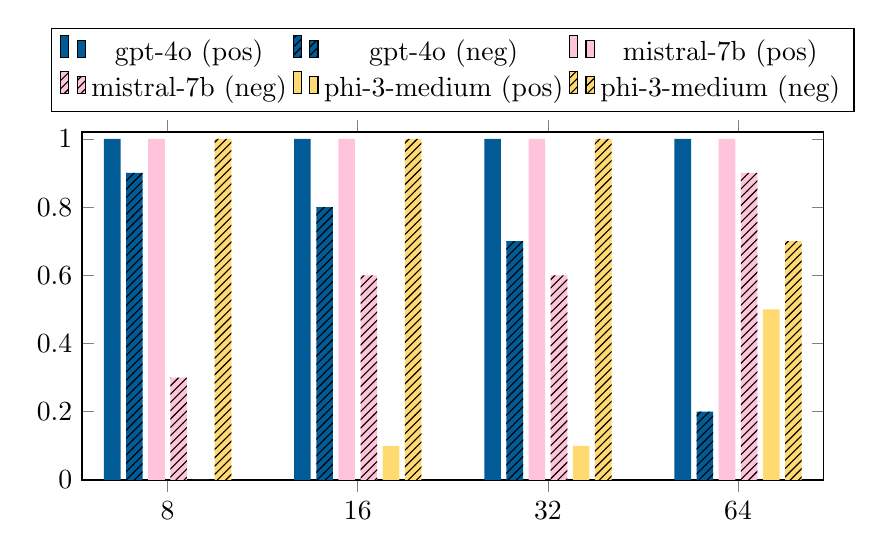
\begin{tikzpicture}
        \begin{axis}[
            ybar,
            bar width=6pt,
            symbolic x coords={8, 16, 32, 64},
            xtick=data,
            ymin=0, ymax=1.02,
            legend columns=3,
            legend style={at={(0.5,1.3)}, anchor=north, draw=black},
            enlarge x limits=0.15,
            width=11cm, height=6cm
        ]
        
        % gpt-4o
        \addplot[fill={rgb,255:red,0;green,91;blue,150}, draw=none] coordinates {(8,1.000) (16,1.000) (32,1.000) (64,1.000)};
        \addlegendentry{gpt-4o (pos)}
        \addplot[fill={rgb,255:red,0;green,91;blue,150}, postaction={
        pattern=north east lines
    }, draw=none] coordinates {(8,0.900) (16,0.800) (32,0.700) (64,0.200)};
        \addlegendentry{gpt-4o (neg)}
        
        % mistral-7b-instruct-v02
        \addplot[fill={rgb,255:red,255;green,196;blue,218}, draw=none] coordinates {(8,1.000) (16,1.000) (32,1.000) (64,1.000)};
        \addlegendentry{mistral-7b (pos)}
        \addplot[fill={rgb,255:red,255;green,196;blue,218}, postaction={
        pattern=north east lines
    }, draw=none] coordinates {(8,0.300) (16,0.600) (32,0.600) (64,0.900)};
        \addlegendentry{mistral-7b (neg)}
        
        % phi-3-medium-128k-instruct
        \addplot[fill={rgb,255:red,255;green,218;blue,112}, draw=none] coordinates {(8,0.000) (16,0.100) (32,0.100) (64,0.500)};
        \addlegendentry{phi-3-medium (pos)}
        \addplot[fill={rgb,255:red,255;green,218;blue,112}, postaction={
        pattern=north east lines
    }, draw=none] coordinates {(8,1.000) (16,1.000) (32,1.000) (64,0.700)};
        \addlegendentry{phi-3-medium (neg)}
        
        \end{axis}
    \end{tikzpicture}}
    \caption{Analysis on \textit{String Search (with subsequence)} across increasing subsequence lengths. This figure examines the behavior of models on \textbf{pos}itive samples (where the subsequence is present) and \textbf{neg}ative samples (where the subsequence is absent).}
    \label{fig:seq_search}
\end{figure}

Figure \ref{fig:seq_search} further analyzes subsequence search performance for GPT-4o, Mistral, and Phi-3-medium. These models exhibit distinct error patterns as the length of the subsequence increases: GPT-4o has no false negative errors (it never misses a present subsequence) but makes more false positive errors as the subsequence length grows, suggesting it overestimates presence in more ambiguous cases.
Mistral also makes no false negative errors but exhibits a decreasing false positive rate, implying it struggles more with shorter distractors. Phi-3-medium, in contrast, makes few false positive errors (rarely identifies an absent sequence as present), but struggles more with false negatives, indicating a general tendency to deny presence. These differing patterns suggest that the models may employ different search strategies, affecting their susceptibility to different types of errors.

For \textit{Batch Search} and \textit{Key-Value Search} tasks (analogous to multi-NIAH and NIAH, respectively), models like Mistral, Phi-3, and Cohere show a notable performance drop, revealing their limitations in handling multiple memory accesses effectively.

% \begin{figure}[h]
%     \centering
%     \begin{subfigure}[t]{0.49\linewidth}
%         \includegraphics[width=\textwidth]{images/recall_black.png}
%         \caption{Black-box models.}
%         \label{fig:first_recall}
%     \end{subfigure}
%     \begin{subfigure}[t]{0.49\linewidth}
%         \includegraphics[width=\textwidth]{images/recall_white.png}
%         \caption{Open-source models.}
%         \label{fig:second_recall}
%     \end{subfigure}
%     \caption{Results for the \textbf{Recall and Edit} tasks.}
%     \label{fig:recall}
% \end{figure}

\begin{figure}[h]
    \centering
    \begin{subfigure}{0.49\columnwidth}
        \resizebox{\textwidth}{!}{
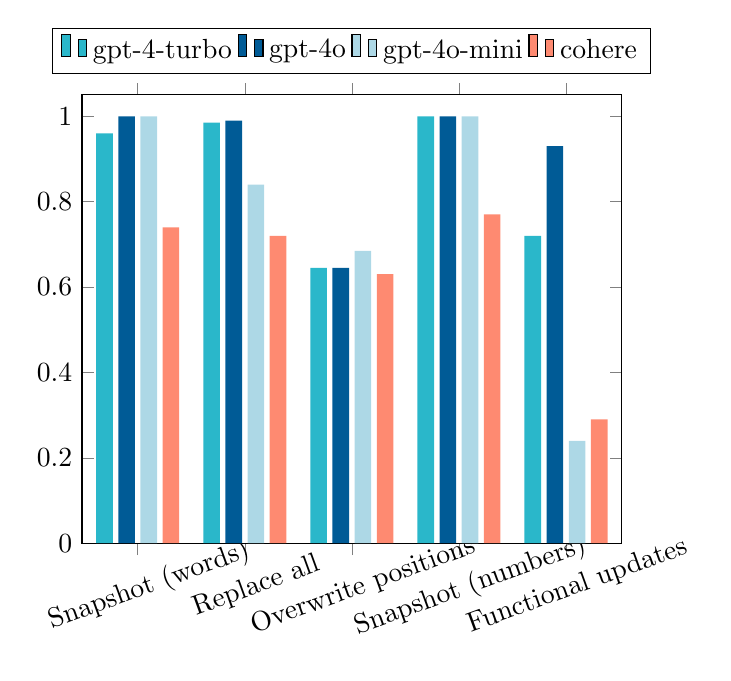
\begin{tikzpicture}
        \begin{axis}[
            ybar,
            bar width=6pt,
            symbolic x coords={Snapshot (words), Replace all, Overwrite positions, Snapshot (numbers), Functional updates},
            xtick=data,
            ymin=0, ymax=1.05,
            legend columns=4,
            legend style={at={(0.5,1.15)}, anchor=north, draw=black},
            enlarge x limits=0.13,
            xticklabel style={rotate=20, anchor=center, yshift=-12pt}
        ]
        
        \addplot[fill={rgb,255:red,42;green,183;blue,202}, draw=none] coordinates {(Snapshot (words),0.96) (Replace all,0.985) (Overwrite positions,0.645) (Snapshot (numbers),1.00) (Functional updates,0.72)};
        \addlegendentry{gpt-4-turbo}
        
        \addplot[fill={rgb,255:red,0;green,91;blue,150}, draw=none] coordinates {(Snapshot (words),1.00) (Replace all,0.99) (Overwrite positions,0.645) (Snapshot (numbers),1.00) (Functional updates,0.93)};
        \addlegendentry{gpt-4o}
        
        \addplot[fill={rgb,255:red,173;green,216;blue,230}, draw=none] coordinates {(Snapshot (words),1.00) (Replace all,0.84) (Overwrite positions,0.685) (Snapshot (numbers),1.00) (Functional updates,0.24)};
        \addlegendentry{gpt-4o-mini}
        
        \addplot[fill={rgb,255:red,254;green,138;blue,113}, draw=none] coordinates {(Snapshot (words),0.74) (Replace all,0.72) (Overwrite positions,0.63) (Snapshot (numbers),0.77) (Functional updates,0.29)};
        \addlegendentry{cohere}
        
        \end{axis}
\end{tikzpicture}}
    \end{subfigure}
    \begin{subfigure}{0.49\columnwidth}
        \resizebox{\textwidth}{!}{    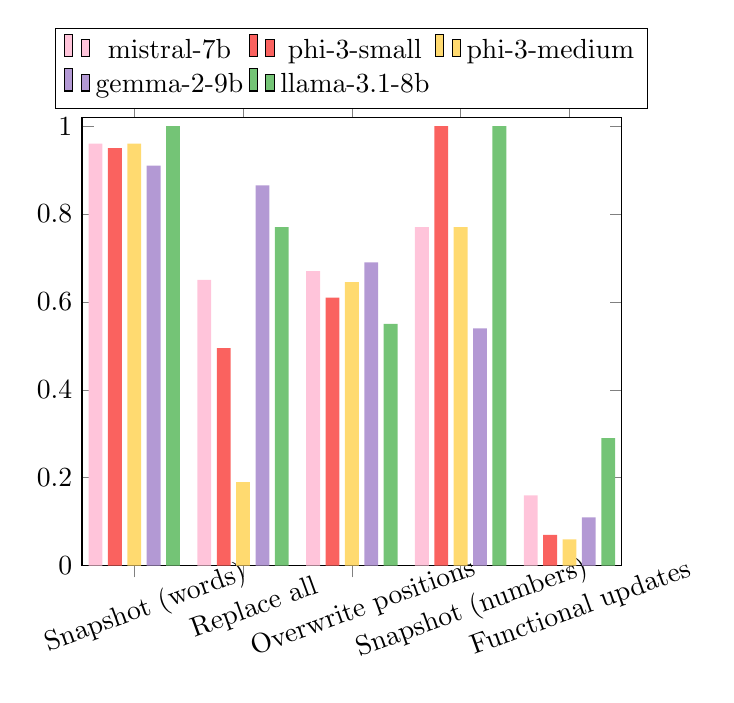
\begin{tikzpicture}
        \begin{axis}[
            ybar,
            bar width=5pt,
            symbolic x coords={Snapshot (words), Replace all, Overwrite positions, Snapshot (numbers), Functional updates},
            xtick=data,
            ymin=0, ymax=1.02,
            legend columns=3,
            legend style={at={(0.5,1.20)}, anchor=north, draw=black},
            enlarge x limits=0.12,
            xticklabel style={rotate=20, anchor=center, yshift=-12pt}
        ]
        
        \addplot[fill={rgb,255:red,255;green,196;blue,218}, draw=none] coordinates {(Snapshot (words),0.96) (Replace all,0.65) (Overwrite positions,0.67) (Snapshot (numbers),0.77) (Functional updates,0.16)};
        \addlegendentry{mistral-7b}
        
        \addplot[fill={rgb,255:red,250;green,98;blue,95}, draw=none] coordinates {(Snapshot (words),0.95) (Replace all,0.495) (Overwrite positions,0.61) (Snapshot (numbers),1.00) (Functional updates,0.07)};
        \addlegendentry{phi-3-small}
        
        \addplot[fill={rgb,255:red,255;green,218;blue,112}, draw=none] coordinates {(Snapshot (words),0.96) (Replace all,0.19) (Overwrite positions,0.645) (Snapshot (numbers),0.77) (Functional updates,0.06)};
        \addlegendentry{phi-3-medium}
        
        \addplot[fill={rgb,255:red,179;green,153;blue,212}, draw=none] coordinates {(Snapshot (words),0.91) (Replace all,0.865) (Overwrite positions,0.69) (Snapshot (numbers),0.54) (Functional updates,0.11)};
        \addlegendentry{gemma-2-9b}
        
        \addplot[fill={rgb,255:red,116;green,196;blue,118}, draw=none] coordinates {(Snapshot (words),1.00) (Replace all,0.77) (Overwrite positions,0.55) (Snapshot (numbers),1.00) (Functional updates,0.29)};
        \addlegendentry{llama-3.1-8b}
        
        \end{axis}
\end{tikzpicture}}
    \end{subfigure}
    \caption{Results for the \textbf{Recall and Edit} tasks.}
    \label{fig:recall}
\end{figure}

\paragraph{Recall and Edit} 
\begin{table}[!h]
    \centering
        \resizebox{0.8\columnwidth}{!}{%
    \begin{tabular}{lllll}
    \toprule
        \textbf{Model} & \textbf{String Search (word)} & \textbf{Snapshot} \\ \hline
gpt-4-turbo    & 1.00 \textcolor{green}{(0.06)} & 1.00 \textcolor{green}{(0.04)} \\ 
gpt-4o         & 1.00 (0.00)                   & 1.00 (0.00)                   \\ 
gpt-4o-mini    & 0.94 \textcolor{red}{(-0.04)}  & 1.00 (0.00)                   \\ 
cohere         & 1.00 (0.00)                   & 1.00 \textcolor{green}{(0.26)} \\ 
mistral-7b     & 1.00 \textcolor{green}{(0.22)} & 0.96 (0.00)                   \\ 
phi-3-small    & 1.00 \textcolor{green}{(0.06)} & 0.99 \textcolor{green}{(0.04)} \\ 
phi-3-medium   & 0.98 \textcolor{red}{(-0.02)}  & 0.87 \textcolor{red}{(-0.09)}  \\ 
gemma-2-9b     & 0.96 \textcolor{red}{(-0.04)}  & 0.96 \textcolor{green}{(0.05)} \\ 
llama-3.1-8b   & 0.98 \textcolor{red}{(-0.02)}  & 1.00 (0.00)                   \\
\bottomrule
    \end{tabular}
    }
    \caption{Ablation study with gibberish context.}
    \label{tab:ablation_gibberish}
\end{table}

Figure \ref{fig:recall} presents the results for the \textbf{Recall and Edit} tasks. While models performed well on basic recall (\textit{Snapshot}), their performance dropped sharply when tasked with making regular edits. A closer analysis of the generated outputs reveals that models struggled with maintaining coherence during edits, often getting trapped in repetitive word loops. For the \textit{Functional Update} task, we deliberately selected simple numerical updates, such as ``Subtract 1 from every number," to ensure the edits were within the models' capabilities. Nevertheless, when comparing performance on \textit{Snapshot (with numbers)} to \textit{Functional Updates}, all models exhibited a steep decline, especially for smaller ones. Analysis of generated outputs revealed that these models frequently deviated from instructions over longer sequences, suggesting difficulties in maintaining consistent rule applications over extended contexts.

Additionally, we conducted a separate ablation study on \textit{Snapshot} and \textit{String Search}. In this study, we replaced meaningful words in the context with gibberish tokens consisting of randomly generated alphabetical characters. As shown in Table \ref{tab:ablation_gibberish}, performance remained largely unchanged, suggesting that semantic meaning was not a significant distractor in these tasks.

\section{Backup: compare with previous works}

\paragraph{Comparison with Theorem 1 of \cite{srikant2024rates}.} While the framework of our proof of Theorem \ref{thm:Srikant-generalize} is mainly inspired by the proof of Theorem 1 of \cite{srikant2024rates}, there are some noteworthy differences. Most importantly, we observe that in the equation beginning from the bottom of Page 7 and continuing to the start of Page 8, the right-most side contains a term
\begin{align}\label{eq:Srikant-error}
-\frac{1}{n-k+1} \mathsf{Tr}\left(\bm{\Sigma}_{\infty}^{-\frac{1}{2}}(\bm{\Sigma}_k - \bm{\Sigma}_{\infty})\bm{\Sigma}_{\infty}^{-\frac{1}{2}}\mathbb{E}[\nabla^2 f(\tilde{\bm{Z}}_k)]\right);
\end{align}
the author argued that ``by taking an expectation to remove conditioning, and defining $\bm{A}_k$ to be $\mathbb{E}[\nabla^2 f(\tilde{\bm{Z}}_k)]$'', this term can be transformed to the term
\begin{align}\label{eq:Srikant-wrong}
-\frac{1}{n-k+1} \mathsf{Tr}\left(\bm{A}_k \left(\bm{\Sigma}_{\infty}^{-\frac{1}{2}} \mathbb{E}[\bm{\Sigma}_k]\bm{\Sigma}_{\infty}^{-\frac{1}{2}}-\bm{I}\right)\right)
\end{align}
in the expression of Theorem 1. However, we note that the function $f(\cdot)$, as defined on Page 6 as the solution to the Stein's equation with respect to $\tilde{h}(\cdot)$, is \emph{dependent on} $\mathcal{F}_{k-1}$; in fact, $f$ corresponds to the function $f_k$ in our proof. Consequently, the terms $\bm{A}_k = \mathbb{E}[\nabla^2 f(\tilde{\bm{Z}}_k)]$ (which is actually a conditional expectation with respect to $\mathcal{F}_{k-1}$), and $\bm{\Sigma}_k$ (which corresponds to $\bm{V}_k$ in our proof), are confounded by $\mathcal{F}_{k-1}$ and hence \emph{not independent}. Therefore, taking expectation, with respect to $\mathcal{F}_0$, on \eqref{eq:Srikant-error} should yield
\begin{align}\label{eq:Srikant-right}
-\frac{1}{n-k+1} \mathbb{E}\left\{\mathsf{Tr}\left(\bm{A}_k \left(\bm{\Sigma}_{\infty}^{-\frac{1}{2}} \bm{\Sigma}_k\bm{\Sigma}_{\infty}^{-\frac{1}{2}}-\bm{I}\right)\right)\right\}
\end{align}
Notice that the expectation is taken over the trace as a whole, instead of only $\bm{\Sigma}_k$. However, also due to the confounding bewteen $\bm{A}_k$ and $\bm{\Sigma}_k$, there is no guarantee that the sum of \eqref{eq:Srikant-right} is bounded as shown in the proof of Theorem 2 in \cite{srikant2024rates} on page 10. In other words, the framework of the proof needs a substantial correction to obtain a meaningful Berry-Esseen bound. 

Our solution in the proof of Theorem \ref{thm:Srikant-generalize} is to replace the matrix $\bm{Q}=\sqrt{n-k+1}\bm{\Sigma}_{\infty}$, as defined on Page 6 of \cite{srikant2024rates}, with the matrix $\bm{P}_k$, following the precedent of \cite{JMLR2019CLT}. This essentially eliminates the term \eqref{eq:Srikant-right}, but would require $\bm{P}_k$ to be measurable with respect to $\mathcal{F}_{k-1}$. For this purpose, we impose the assumption that $\bm{P}_1 = n\bm{\Sigma}_n$ almost surely, also following the precedent of \cite{JMLR2019CLT}. The relaxation of this assumption would be addressed in Theorem \ref{thm:Berry-Esseen-mtg}. 

Another important improvement we made in Theroem \ref{thm:Srikant-generalize} is to tighten the upper bound through a closer scrutiny of the smoothness of the solution to the Stein's equation, as is indicated in Proposition \ref{prop:Stein-smooth}. This paves the way for Corollary \ref{cor:Wu}, the proof of which we present in the next subsection. 


\begin{table}[!htbp] \centering
  \caption{Human Choices and Predictions About GenAI Choice in the Same Problem: Heterogeneity by Exposure and Attitudes (Pooled)}
\begin{adjustbox}{scale=0.8}
\begin{tabular}{@{\extracolsep{5pt}}lccccc}
% \\[-1.8ex]\hline
% \hline \\[-1.8ex]
\toprule
& \multicolumn{5}{c}{\textit{Dependent variable: Prediction}} \
\cr \cline{2-6}
\\[-1.8ex] & \multicolumn{1}{c}{Heavy User} & \multicolumn{1}{c}{Text-Based LLM User} & \multicolumn{1}{c}{Paid User} & \multicolumn{1}{c}{Agree AI Similar} & \multicolumn{1}{c}{Agree AI Better}  \\
\\[-1.8ex] & (1) & (2) & (3) & (4) & (5) \\
% \hline \\[-1.8ex]
\midrule
 X$\times$Heavy User & -0.056$^{}$ & & & & \\
& (0.052) & & & & \\
 X$\times$Text-Based LLM User & & 0.082$^{**}$ & & & \\
& & (0.040) & & & \\
 X$\times$Paid User & & & -0.001$^{}$ & & \\
& & & (0.072) & & \\
 X$\times$Agree AI Similar & & & & 0.033$^{}$ & \\
& & & & (0.045) & \\
 X$\times$Agree AI Better & & & & & 0.019$^{}$ \\
& & & & & (0.017) \\
 Problem FE & Yes & Yes & Yes & Yes & Yes \\
 X$\times$Problem FE & Yes & Yes & Yes & Yes & Yes \\
 G$\times$Problem FE & Yes & Yes & Yes & Yes & Yes \\
% \hline \\[-1.8ex]
\midrule
 Observations & 2700 & 2700 & 2700 & 2700 & 2700 \\
 % Residual Std. Error & 22.874 & 22.851 & 22.863 & 22.847 & 22.895 \\
% \hline
% \hline \\[-1.8ex]
\bottomrule
\textit{Note:} & \multicolumn{5}{r}{Standard errors are clustered at the problem level. $^{*}$p$<$0.1; $^{**}$p$<$0.05; $^{***}$p$<$0.01} \\
% \multicolumn{6}{r}\textit{} \\
\end{tabular}
\end{adjustbox}
\label{tab:group} \end{table}


\paragraph{Match and Compare}
 As shown in Figure \ref{fig:match}, model performance in the \textbf{Match and Compare} tasks was relatively consistent across different model sizes. Given that counting is a well-known weakness in LLMs, it is unsurprising that all models struggled significantly with the counting task, though GPT models performed slightly better than others. However, models generally succeeded in identifying the duplicates (in \textit{Find duplicates}), and primarily struggled with the counting aspect -- which requires tracking and updating an integer state, a skill that is more similar to stateful processing. This suggests that relying solely on counting-based tests \cite{song2024countingstars} could overly bias the evaluation and fail to capture broader model capabilities. The results also indicate that models exhibit some ability to recognize relative positions and group associations, but their accuracy remains limited (ranging between 0.6-0.8). A closer examination of model generations reveals an overwhelming tendency for the models to produce false positive errors -- models often answer “yes” when the correct answer is “no”, while making very few false negative errors. This means that when the relationship is correct, the models can more reliably identify it. This may stem from a combination of their inherent inclination to agree and the difficulty in recognizing relative comparisons and associations.

% \begin{figure}[h]
%     \centering
%     \includegraphics[width=0.92\columnwidth]{images/difference.png}
%     \caption{Results for \textbf{Spot the Differences }tasks.}
%     \label{fig:difference}
% \end{figure}

\begin{figure}[h]
\centering
\resizebox{0.9\columnwidth}{!}{
 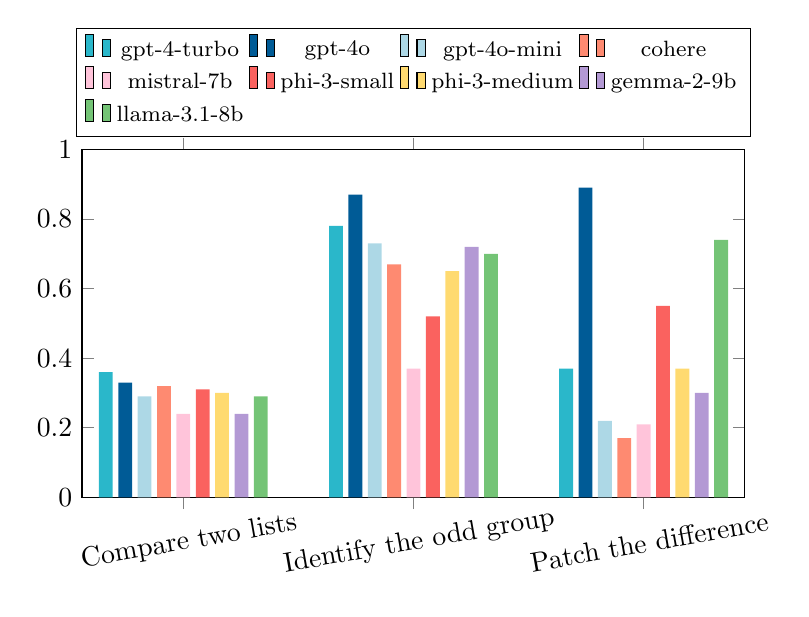
\begin{tikzpicture}
        \begin{axis}[
            ybar,
            bar width=5pt,
            symbolic x coords={Compare two lists, Identify the odd group, Patch the difference},
            xtick=data,
            ymin=0, ymax=1.0,
            legend columns=4,
            legend style={at={(0.5,1.35)}, anchor=north, draw=black, font=\footnotesize},
            enlarge x limits=0.22,
            xticklabel style={rotate=10, anchor=center, yshift=-12pt},
            width=10cm, height=6cm,
        ]
        
        \addplot[fill={rgb,255:red,42;green,183;blue,202}, draw=none] coordinates {(Compare two lists,0.36) (Identify the odd group,0.78) (Patch the difference,0.37)};
        \addlegendentry{gpt-4-turbo}
        
        \addplot[fill={rgb,255:red,0;green,91;blue,150}, draw=none] coordinates {(Compare two lists,0.33) (Identify the odd group,0.87) (Patch the difference,0.89)};
        \addlegendentry{gpt-4o}
        
        \addplot[fill={rgb,255:red,173;green,216;blue,230}, draw=none] coordinates {(Compare two lists,0.29) (Identify the odd group,0.73) (Patch the difference,0.22)};
        \addlegendentry{gpt-4o-mini}
        
        \addplot[fill={rgb,255:red,254;green,138;blue,113}, draw=none] coordinates {(Compare two lists,0.32) (Identify the odd group,0.67) (Patch the difference,0.17)};
        \addlegendentry{cohere}
        
        \addplot[fill={rgb,255:red,255;green,196;blue,218}, draw=none] coordinates {(Compare two lists,0.24) (Identify the odd group,0.37) (Patch the difference,0.21)};
        \addlegendentry{mistral-7b}
        
        \addplot[fill={rgb,255:red,250;green,98;blue,95}, draw=none] coordinates {(Compare two lists,0.31) (Identify the odd group,0.52) (Patch the difference,0.55)};
        \addlegendentry{phi-3-small}
        
        \addplot[fill={rgb,255:red,255;green,218;blue,112}, draw=none] coordinates {(Compare two lists,0.30) (Identify the odd group,0.65) (Patch the difference,0.37)};
        \addlegendentry{phi-3-medium}
        
        \addplot[fill={rgb,255:red,179;green,153;blue,212}, draw=none] coordinates {(Compare two lists,0.24) (Identify the odd group,0.72) (Patch the difference,0.30)};
        \addlegendentry{gemma-2-9b}
        
        \addplot[fill={rgb,255:red,116;green,196;blue,118}, draw=none] coordinates {(Compare two lists,0.29) (Identify the odd group,0.70) (Patch the difference,0.74)};
        \addlegendentry{llama-3.1-8b}
        
        \end{axis}
    \end{tikzpicture}}
    \caption{Results for \textbf{Spot the Differences }tasks.}
    \label{fig:difference}
\end{figure}

\paragraph{Spot the Differences}
As shown in Figure \ref{fig:difference}, performance across all models are poor on \textit{Compare Two Lists}, suggesting inherent difficulties in cross-referencing information across long contexts, even for larger models.  GPT-4o and the LLaMA model significantly outperform the others in the \textit{Identify the Odd Group} task, highlighting a general weakness in detecting contextual differences by the other models. However, an 8B LLaMA model outperforms both equivalently-sized models and even GPT-4 in this task, suggesting that model size alone was not the determining factor. This indicates that architectural differences, training objectives, or specific inductive biases may contribute to improved performance in comparative memory utilization.


\paragraph{Compute on Sets and Lists}
The tasks in this category require models to recognize and process group structures within the context, and performance gradually declines as the complexity of the task increases (see Table \ref{tab:lists}). For instance, in comparing the \textit{Group Membership} task with the \textit{String Search} task, where the former requires identifying which list a word belongs to rather than simply determining its presence, the performance of open-source models drops considerably. Similarly, in comparing the \textit{Group Association} task with the \textit{Group Membership} task, where the former requires determining whether two words belong to the same group, all models exhibit a noticeable decline in performance. The decline becomes even more pronounced when comparing the \textit{ Group Association (alternating)} variant of the task to the standard \textit{Group Association} task. Here, the context involves alternating repeated groups rather than simple group structures, which further challenges the models' abilities to handle partitioned contexts effectively.

An interesting observation was found during the \textit{Iterate} task. In an ablation study, we modified the task to require returning the first words in each list instead of the last words (making it more similar to the \textit{Batch Search} task). The performance sharply declines when models are asked to return the last words, despite their strong information-fetching capabilities. This suggests that, while the models can retrieve information effectively, they struggle to accurately recognize and process partitions within the context.


\begin{table}[h!]
\large
\centering
\begin{adjustbox}{width=\columnwidth} % Automatically fit within column width
\begin{tabular}{|c|p{0.75\columnwidth}|} % Adjust the second column width proportionally
\hline
\textbf{Symbol} & \textbf{Explanation} \\ \hline
$q^{\text{obj}} \in SE(2)$ & Object pose \\ \hline
$q^{\text{robot}} \in \mathbb{R}^9$ & Robot configuration (9 DoF robot joint position) \\ \hline
$q^{\text{obj}}_\text{sg} \in SE(2)$ & Subgoal object pose \\ \hline
$q^{\text{robot}}_\text{sg} \in SE(3) \times \mathbb{R}^3$ & Subgoal robot configuration (End-effector pose in $SE(3)$ and gripper tip positions in 3D space) \\ \hline
$q^{\text{obj}}_{\text{init}} \in SE(2)$ & Initial object pose of the task \\ \hline
$q^{\text{robot}}_{\text{init}} \in \mathbb{R}^9$ & Initial robot configuration of the task (9 DoF robot joint position) \\ \hline
$q^{\text{obj}}_{\text{goal}} \in SE(2)$ & Goal object pose of the task \\ \hline
$s$ & State \\ \hline
% $sg$ & Subgoal information (e.g., subgoal object pose, robot configuration) \\ \hline
\end{tabular}
\end{adjustbox}
\caption{Notation table for task parameters}
\label{tab:state_notation}
\end{table}

\paragraph{Stateful Processing}

\begin{figure}[t!]
    \centering
    \begin{subfigure}{0.49\columnwidth}
        \resizebox{\textwidth}{!}{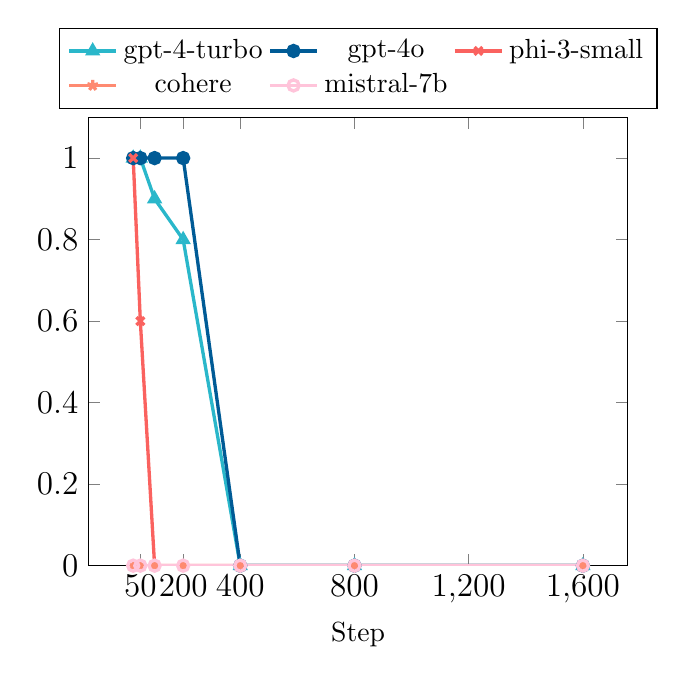
\begin{tikzpicture}
    \begin{axis}[
        xlabel={Step},
        legend style={at={(0.5,1.2)}, anchor=north, cells={align=left}, legend columns=3},
        ymin=0, ymax=1.1,
        xtick={50, 200, 400, 800, 1200, 1600},
        ytick={0,0.2,0.4,0.6,0.8,1.0},
        grid=none,
        tick label style={font=\large}
    ]

    % GPT-4-Turbo
    \addplot[mark=triangle, very thick, color={rgb,255:red,42;green,183;blue,202}] coordinates {
        (25,1.0) (50,1.0) (100,0.9) (200,0.8) (400,0.0) (800,0.0) (1600,0.0)
    };
    \addlegendentry{gpt-4-turbo}

    % GPT-4o
    \addplot[mark=*, very thick, color={rgb,255:red,0;green,91;blue,150}] coordinates {
        (25,1.0) (50,1.0) (100,1.0) (200,1.0) (400,0.0) (800,0.0) (1600,0.0)
    };
    \addlegendentry{gpt-4o}



    % Phi-3-Small
    \addplot[mark=x, very thick, color={rgb,255:red,250;green,98;blue,95}] coordinates {
        (25,1.0) (50,0.6) (100,0.0) (200,0.0) (400,0.0) (800,0.0) (1600,0.0)
    };
    \addlegendentry{phi-3-small}

    % Cohere
    \addplot[mark=star, very thick, color={rgb,255:red,254;green,138;blue,113}] coordinates {
        (25,0.0) (50,0.0) (100,0.0) (200,0.0) (400,0.0) (800,0.0) (1600,0.0)
    };
    \addlegendentry{cohere}

    % Mistral-7B
    \addplot[mark=o, very thick, color={rgb,255:red,255;green,196;blue,218}] coordinates {
        (25,0.0) (50,0.0) (100,0.0) (200,0.0) (400,0.0) (800,0.0) (1600,0.0)
    };
    \addlegendentry{mistral-7b}
    
    \end{axis}
\end{tikzpicture}}
    \end{subfigure}
    \begin{subfigure}{0.49\columnwidth}
        \resizebox{\textwidth}{!}{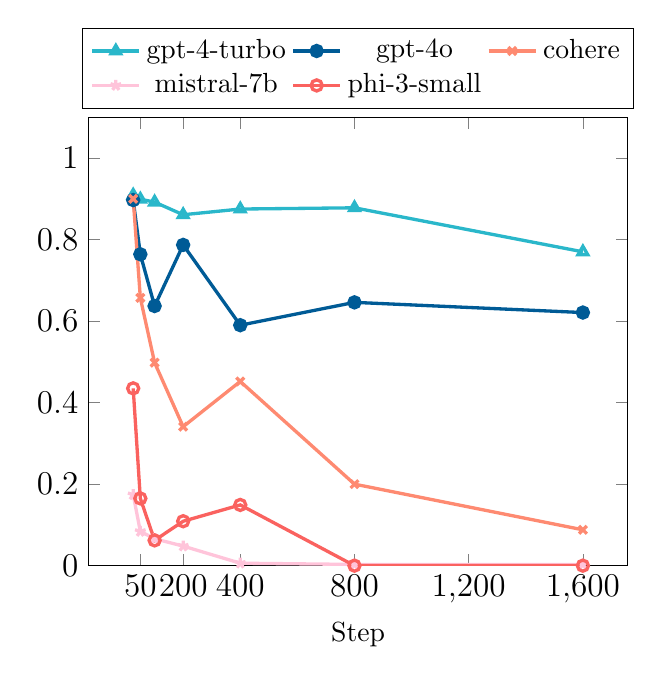
\begin{tikzpicture}
    \begin{axis}[
        xlabel={Step},
        legend style={at={(0.5,1.2)}, anchor=north, cells={align=left}, legend columns=3},
        ymin=0, ymax=1.1,
        xtick={50, 200, 400, 800, 1200, 1600},
        ytick={0,0.2,0.4,0.6,0.8,1.0},
        grid=none,
        tick label style={font=\large}
    ]

    % GPT-4-Turbo
    \addplot[mark=triangle, very thick, color={rgb,255:red,42;green,183;blue,202}] coordinates {
        (25,0.909) (50,0.899) (100,0.892) (200,0.861) (400,0.875) (800,0.878) (1600,0.770)
    };
    \addlegendentry{gpt-4-turbo}

    % GPT-4o
    \addplot[mark=*, very thick, color={rgb,255:red,0;green,91;blue,150}] coordinates {
        (25,0.897) (50,0.764) (100,0.637) (200,0.787) (400,0.590) (800,0.646) (1600,0.621)
    };
    \addlegendentry{gpt-4o}

    % Cohere
    \addplot[mark=x, very thick, color={rgb,255:red,254;green,138;blue,113}] coordinates {
        (25,0.900) (50,0.657) (100,0.498) (200,0.341) (400,0.452) (800,0.200) (1600,0.088)
    };
    \addlegendentry{cohere}

    % Mistral-7B
    \addplot[mark=star, very thick, color={rgb,255:red,255;green,196;blue,218}] coordinates {
        (25,0.174) (50,0.084) (100,0.066) (200,0.048) (400,0.006) (800,0.003) (1600,0.003)
    };
    \addlegendentry{mistral-7b}

    % Phi-3-Small
    \addplot[mark=o, very thick, color={rgb,255:red,250;green,98;blue,95}] coordinates {
        (25,0.435) (50,0.165) (100,0.062) (200,0.109) (400,0.149) (800,0.000) (1600,0.000)
    };
    \addlegendentry{phi-3-small}
    
    \end{axis}
\end{tikzpicture}}
    \end{subfigure}
    \caption{Ablation study on the number of operation steps for the \textbf{quantity state} (left) and\textbf{ set state }(right).}
    \label{fig:ablation_state_step}
\end{figure}



Table \ref{tab:state} presents the results for the \textbf{Stateful Processing} tasks, where performance gaps among models are the most pronounced. The GPT-4(o) models perform well on integer state tracking, while most other models struggle (near zero accuracy). For set state tracking, larger models generally perform better.

We conducted an ablation study to examine how the number of operation steps influences performance of five selected models (Fig. \ref{fig:ablation_state_step}). For quantity state tracking, GPT-4(o) models perform well within fewer than 200 steps but experience a sharp decline in accuracy beyond this threshold. For set state tracking, the performance decline is more gradual. The differences in performance drop between the two tasks can be attributed to the nature of the two tasks. While tracking an integer state might seem simpler than tracking a set, it actually requires the model to maintain and apply every operation sequentially to compute the final value. In contrast, for set state, the fixed size of the set makes more recent operations more relevant to the final state, reducing the need for exhaustive step-by-step tracking. Nevertheless, even in this scenario, all models show a clear inability to handle longer or more complex operation sequences effectively. Interestingly, GPT-4 model outperformed GPT-4o at this task, suggesting potential optimization trade-offs may have affected its ability to manage set-based updates. 

Overall, while larger models like GPT-4(o) exhibit some ability to track state over time, their effectiveness rapidly deteriorates as task complexity increases. Smaller models, in particular, struggle to track operations over time, pointing to significant gaps in their ability to manage and process sequential dependencies critical for state tracking tasks.

\subsection{Results on Composite Tests}

\section{Simple Construction of Projective Compositions}
\label{sec:comp_coord}

It is not clear apriori that projective compositional distributions satisfying Definition \ref{def:proj_comp} ever exist, much less that there is any straightforward way to sample from them.
To explore this, we first restrict attention to perhaps the simplest setting, where the projection functions $\{\Pi_i\}$ are
just coordinate restrictions.
This setting is meant to generalize the intuition we had
in the CLEVR example of Figure~\ref{fig:len_gen},
where different objects were composed in disjoint regions of the image.
We first define the construction of the composed distribution,
and then establish its theoretical properties.








\subsection{Defining the Construction}
Formally, suppose we have a set of distributions
$(p_1, p_2, \ldots, p_k)$ that we wish to compose;
in our running CLEVR example, each $p_i$ is the distribution of images
with a single object at position $i$.
Suppose also we have some reference distribution $p_b$,
which can be arbitrary, but should be thought of as a 
``common background'' to the $p_i$s.
Then, one popular way to construct a composed distribution
is via the \emph{compositional operator} defined below.
(A special case of this construction is used in \citet{du2023reduce}, for example).


\begin{definition}[Composition Operator]
    \label{def:comp_oper}
    Define the \emph{composition operator} $\cC$ acting on an arbitrary set of distributions $(p_b, p_1, p_2, \ldots)$ by
    \begin{align}
    \label{eq:comp_oper}
    \cC[\vec{p}] := \cC[p_b, p_1, p_2, \dots](x) := \frac{1}{Z} p_b(x) \prod_i \frac{p_i(x)}{p_b(x)},
    \end{align}
    where $Z$ is the appropriate normalization constant. We name $\cC[\vec{p}]$ the \emph{composed distribution}, and the score of $\cC[\vec{p}]$ the \emph{compositional score}:
    \begin{align}
    \label{eqn:comp_score}
    &\grad_x \log \cC[\vec{p}](x)  \\
    &= \grad_x \log p_b(x) + \sum_i \left( \grad_x \log p_i(x) - \grad_x \log p_b(x) \right). \notag
    \end{align}
\end{definition}
Notice that if $p_b$ is taken to be the unconditional distribution then this is exactly the Bayes-composition.


\vspace{-0.5em}
\subsection{When does the Composition Operator Work?}
We can always apply the composition operator to any set of distributions,
but when does this actually yield a ``correct'' composition
(according to Definition~\ref{def:proj_comp})?
One special case is when each distribution $p_i$ is
``active'' on a different, non-overlapping set of coordinates.
We formalize this property below
as \emph{Factorized Conditionals} (Definition~\ref{def:factorized}).
The idea is, 
each distribution $p_i$
must have a particular set of ``mask'' coordinates $M_i \subseteq [n]$ which it
samples in a characteristic way,
while independently sampling all other coordinates
from a common background distribution.
If a set of distributions $(p_b, p_1, p_2, \ldots)$ has this
\emph{Factorized Conditional} structure, then 
the composition
operator will produce a projective composition (as we will prove below).



\begin{definition}[Factorized-Conditionals]
\label{def:factorized}

We say a set of distributions $(p_b, p_1, p_2, \dots p_k)$
over $\R^n$
are \emph{Factorized Conditionals} if
there exists a partition of coordinates $[n]$
into disjoint subsets $M_b, M_1, \dots M_k$ such that:
\begin{enumerate}
    \setlength{\itemsep}{1pt}
    \item $(x|_{M_i}, x|_{M_i^c})$ are independent under $p_i$.
    \item $(x|_{M_b}, x|_{M_1}, x|_{M_2}, \dots, x|_{M_k})$
    are mutually independent under $p_b$.
    \item $p_i(x|_{M_i^c}) = p_b(x|_{M_i^c})$.
\end{enumerate}

Equivalently, if we have:
\begin{align}
    p_i(x) &= p_i(x|_{M_i}) p_b(x|_{M_i^c}), \text{ and} \label{eqn:cc-cond}\\
    p_b(x) &= p_b(x|_{M_b}) \prod_{i \in [k]} p_b(x|_{M_i}). \notag
\end{align}
\end{definition}
\vspace{-1em}
Equation~\eqref{eqn:cc-cond} means that each $p_i$
can be sampled by first sampling $x \sim p_b$,
and then overwriting the coordinates of $M_i$
according to some other distribution (which can be specific to distribution $i$).
For instance, the experiment of Figure~\ref{fig:len_gen}
intuitively satisfies this property, since 
each of the conditional distributions could essentially be sampled
by first sampling an empty background image ($p_b$), then ``pasting''
a random object in the appropriate location (corresponding to pixels $M_i$).
If a set of distributions obey this Factorized Conditional structure,
then we can prove that the composition operator $\cC$
yields a correct projective composition,
and reverse-diffusion correctly samples from it.
Below, let $N_t$ denote the noise operator of the
diffusion process\footnote{Our results are agnostic to the specific diffusion noise-schedule and scaling used.} at time $t$.

\begin{theorem}[Correctness of Composition]
\label{lem:compose}
Suppose a set of distributions $(p_b, p_1, p_2, \dots p_k)$
satisfy Definition~\ref{def:factorized},
with corresponding masks $\{M_i\}_i$.
Consider running the reverse-diffusion SDE 
using the following compositional scores at each time $t$:
\begin{align}
s_t(x_t) &:= \grad_x \log \cC[p_b^t, p_1^t, p_2^t, \ldots](x_t),
\end{align}
where $p_i^t := N_t[p_i]$ are the noisy distributions.
Then, the distribution of the generated sample $x_0$ at time $t=0$ is:
\begin{align}
\label{eqn:p_hat}
\hat{p}(x) := p_b(x|_{M_b}) \prod_i p_i(x|_{M_i}).
\end{align}
In particular,
$\hat{p}(x|_{M_i}) = p_i(x|_{M_i})$ for all $i$,
and so
$\hat{p}$ is a projective composition
with respect to projections $\{\Pi_i(x) := x|_{M_i}\}_i$,
per Definition \ref{def:proj_comp}.
\end{theorem}




Unpacking this, Line \ref{eqn:p_hat} says that the final generated distribution
$\hat{p}(x)$ can be sampled by
first sampling
the coordinates $M_b$ according to $p_b$ (marginally),
then independently sampling 
coordinates $M_i$ according to $p_i$ (marginally) for each $i$.
Similarly, by assumption, $p_i(x)$ can be sampled by first sampling the coordinates $M_i$ in some specific way, and then independently sampling the remaining coordinates according to $p_b$. Therefore Theorem \ref{lem:compose} says that $\hat{p}(x)$ samples the coordinates \emph{$M_i$ exactly as they would be sampled by $p_i$}, for each $i$ we wish to compose. 

\begin{proof}(Sketch) \small
Since $\vec{p}$ satisfies Definition \ref{def:factorized}, we have
\begin{align*}
&\cC[\vec{p}](x) := p_b(x) \prod_i \frac{p_i(x)}{p_b(x)} \notag 
= p_b(x) \prod_i \frac{p_b(x_t|_{M_i^c}) p_i(x|_{M_i})}{p_b(x|_{M_i^c})p_b(x|_{M_i})} \notag \\
&= p_b(x) \prod_i \frac{p_i(x|_{M_i})}{p_b(x|_{M_i})} \notag 
= p_b(x|_{M_b}) \prod_i p_i(x_t|_{M_i}) := \hat{p}(x).
\end{align*}
The sampling guarantee follows from the commutativity of composition with the diffusion noising process, i.e. $\cC[\vec{p^t}]= N_t[\cC[\vec{p}]]$. 
The complete proof is in Appendix \ref{app:compose_pf}.
\end{proof}

\begin{remark}
In fact, Theorem~\ref{lem:compose} still holds under any orthogonal transformation of the variables,
because the diffusion noise process commutes with orthogonal transforms.
We formalize this as Lemma~\ref{lem:orthogonal_sampling}.
\end{remark}

\begin{remark}
Compositionality is often thought of in terms of orthogonality between scores.
Definition \ref{def:factorized} implies orthogonality between the score differences that appear in the composed score \eqref{eqn:comp_score}:
$\grad_x \log p_i^t(x_t) - \grad_x \log p_b^t(x_t),$
but the former condition is strictly stronger
(c.f. Appendix \ref{app:score_orthog}).
\end{remark}

\begin{remark}
Notice that the composition operator $\cC$
can be applied to a set of Factorized Conditional
distributions
without knowing the coordinate partition $\{M_i\}$.
That is, we can compose distributions and compute scores
without knowing apriori exactly ``how'' these distributions are supposed to compose
(i.e. which coordinates $p_i$ is active on).
This is already somewhat remarkable, and we will see a much
stronger version of this property in the next section.
\end{remark}

\textbf{Importance of background.}
Our derivations highlight the crucial role of the background
distribution $p_b$ for the composition operator  
(Definition~\ref{def:comp_oper}).
While prior works have taken $p_b$ to be an unconditional distribution and the $p_i$'s its associated conditionals,
our results suggest this is not always the optimal choice -- in particular,
it may not satisfy a Factorized Conditional structure (Definition~\ref{def:factorized}). Figure~\ref{fig:len_gen_monster} demonstrates this empirically: settings (a) and (b) attempt to compose the same distributions using different backgrounds -- empty (a) or unconditional (b) -- with very different results.

\subsection{Approximate Factorized Conditionals in CLEVR.}
\label{sec:clevr-details}

In \cref{fig:len_gen_monster} we explore compositional length-generalization (or lack thereof) in three different setting, two of which (\cref{fig:len_gen_monster}a and \ref{fig:len_gen_monster}c) approximately satisfy \cref{def:factorized}. In this section we explicitly describe how our definition of Factorized Conditionals approximately captures the CLEVR settings of Figures \ref{fig:len_gen_monster}a and \ref{fig:len_gen_monster}c. The setting of \ref{fig:len_gen_monster}b does not satisfy our conditions, as discussed in \cref{sec:problematic-compositions}.

\textbf{Single object distributions with empty background.}
This is the setting of both \cref{fig:len_gen} and \cref{fig:len_gen_monster}a.
The background distribution $p_b$ 
over $n$ pixels is images of an empty scene with no objects.
For each $i \in \{1,\ldots,L\}$ (where $L=4$ in \cref{fig:len_gen} and $L=9$ in \cref{fig:len_gen_monster}a), define the set $M_i \subset [n]$ 
as the set of pixel indices surrounding location $i$.
($M_i$ should be thought of as a ``mask'' that
that masks out objects at location $i$).
Let $M_b := (\cup_i M_i)^c$ be the remaining
pixels in the image.
Then, we claim the distributions $(p_b, p_1, \ldots, p_L)$
form approximately
Factorized Conditionals, with corresponding
coordinate partition $\{M_i\}$.
This is essentially because each distribution $p_i$
matches the background $p_b$ on all pixels except those surrounding
location $i$ (further detail in Appendix~\ref{app:clevr-details}).
Note, however, that the conditions of Definition~\ref{def:factorized}
do not \emph{exactly} hold in the experiment of Figure~\ref{fig:len_gen} -- there is still some dependence between
the masks $M_i$, since objects can cast shadows or even occlude each other.
Empirically, these deviations 
have greater impact
when composing many objects, as seen in \cref{fig:len_gen_monster}a.


\textbf{Bayes composition with cluttered distributions.}
In \cref{fig:len_gen_monster}c we replicate CLEVR experiments in  \citet{du2023reduce, liu2022compositional} where the images contain many objects (1-5) and the conditions label the location of one randomly-chosen object. It turns out the unconditional together with the conditionals can approximately act as Factorized Conditionals in ``cluttered'' settings like this one. The intuition is that if the conditional distributions each contain one specific object plus many independently sampled random objects (``clutter''), then the unconditional distribution \emph{almost} looks like independently sampled random objects, which together with the conditionals \emph{would} satisfy Definition \ref{def:factorized} (further discussion in Appendix \ref{app:clevr-details} and \ref{app:bayes_connect}). This helps to explain the length-generalization observed in \citet{liu2022compositional} and verified in our experiments (\cref{fig:len_gen_monster}c).







\section{Projective Composition in Feature Space}
\label{sec:comp_feature}

\begin{figure}
    \centering
    \includegraphics[width=1.0\linewidth]{figures/feat-space-vis.png}
    \caption{A commutative diagram illustrating Theorem~\ref{lem:transform_comp}.
    Performing composition in pixel space is equivalent 
    to encoding into a feature space ($\cA$),
    composing there,
    and decoding back
    to pixel space ($\cA^{-1}$).
    }
    \label{fig:feat-space-vis}
\end{figure}

So far we have focused on the setting where the projection functions $\Pi_i$ are simply projections onto coordinate subsets $M_i$ in the native space (e.g. pixel space).
This covers simple examples like Figure~\ref{fig:len_gen} but does not include more realistic situations such as Figure~\ref{fig:style-content},
where the properties to be composed are more abstract.
For example a property like ``oil painting'' does not correspond to projection
onto a specific subset of pixels in an image.
However, we may hope that there exists some conceptual feature space
in which ``oil painting'' does correspond to a particular subset of variables.
In this section, we extend our results to the case where the composition occurs in some conceptual feature space, and each distribution to be composed
corresponds to some particular subset of \emph{features}.


Our main result is a featurized analogue of Theorem~\ref{lem:compose}:
if there exists \emph{any} invertible transform $\cA$
mapping into a feature space
where Definition \ref{def:factorized} holds,
then the composition operator (Definition~\ref{def:comp_oper})
yields a projective composition in this feature space, as shown in Figure~\ref{fig:feat-space-vis}.

\begin{theorem}[Feature-space Composition]
\label{lem:transform_comp}
Given distributions $\vec{p} := (p_b, p_1, p_2, \dots p_k)$,
suppose there exists a diffeomorphism $\cA: \R^n \to \R^n$
such that
$(\cA \sharp p_b, \cA \sharp p_1, \dots \cA \sharp p_k)$
satisfy Definition~\ref{def:factorized},
with corresponding partition $M_i \subseteq [n]$.
Then, the composition $\hat{p} := \cC[\vec{p}]$ satisfies:
\begin{align}
\label{eqn:p_hat_A}
\cA \sharp \hat{p}(z)
\equiv
(\cA \sharp p_b (z))|_{M_b} \prod_{i=1}^k (\cA \sharp p_i(z))|_{M_i}.
\end{align}
Therefore, $\hat{p}$
is a projective composition of $\vec{p}$ w.r.t. projection functions
$\{\Pi_i(x) := \cA(x)|_{M_i}\}$.
\end{theorem}
This theorem is remarkable because it means we can
compose distributions $(p_b, p_1, p_2, \dots)$ in the base space,
and this composition will ``work correctly'' in the feature space
automatically (Equation~\ref{eqn:p_hat_A}),
without us ever needing to compute or even know the feature transform $\cA$
explicitly.



Theorem~\ref{lem:transform_comp} may apriori seem too strong
to be true, since it somehow holds for all feature spaces $\cA$
simultaneously.
The key observation underlying Theorem~\ref{lem:transform_comp} 
is that the composition operator $\cC$ behaves
well under reparameterization.
\begin{lemma}[Reparameterization Equivariance]
\label{lem:reparam}
The composition operator of Definition~\ref{def:comp_oper}
is reparameterization-equivariant. That is,
for all diffeomorphisms $\cA: \R^n \to \R^n$
and all tuples of distributions $\vec{p} = (p_b, p_1, p_2, \dots, p_k)$,
\begin{align}
 \cC[ \cA \sharp \vec{p}] =  \cA \sharp \cC[\vec{p}].
\end{align}
\end{lemma}
\arxiv{\footnote{
For example (separate from our goals in this paper):
Classifier-Free-Guidance can be seen as an instance of the composition operator.
Thus, Lemma~\ref{lem:reparam} implies that performing CFG
in latent space is \emph{equivalent} to CFG in pixel-space,
assuming accurate score-models in both cases.}}
\arxiv{This lemma is potentially of independent interest:
reparametrization-equivariance
is a very strong property which is typically not satisfied by
standard operations between probability distributions---
for example, the ``simple product'' $p_1(x)p_2(x)$ does not satisfy it---
so it is mathematically notable that the composition operator 
has this structure.
Lemma~\ref{lem:reparam} and Theorem~\ref{lem:transform_comp}
are proved in Appendix \ref{app:param-indep}.}

This lemma is potentially of independent interest:
equivariance distinguishes the composition operator
from many other common operators
(e.g. the simple product).
Lemma ~\ref{lem:reparam} and Theorem~\ref{lem:transform_comp}
are proved in Appendix \ref{app:param-indep}.

\section{Sampling from Compositions.}
The feature-space Theorem~\ref{lem:transform_comp} is weaker than Theorem~\ref{lem:compose}
in one important way: it does not provide a sampling algorithm.
That is, Theorem~\ref{lem:transform_comp} guarantees that $\hat{p} := \cC[\vec{p}]$
is a projective composition, but does not guarantee that reverse-diffusion
is a valid sampling method.

There is one special case where diffusion sampling \emph{is} guaranteed to work, namely, for orthogonal transforms (which can seen as a straightforward extension of the coordinate-aligned case of \cref{lem:compose}):
\begin{lemma}[Orthogonal transform enables diffusion sampling]
\label{lem:orthogonal_sampling}
If the assumptions of Lemma \ref{lem:transform_comp} hold for $\cA(x) = Ax$, where $A$ is an orthogonal matrix, then running a reverse diffusion sampler with scores $s_t = \grad_x \log \cC[\vec{p}^t]$ generates the composed distribution $\hat{p} = \cC[\vec{p}]$ satisfying \eqref{eqn:p_hat_A}.
\end{lemma}
The proof is given in \cref{app:orthog_sample_pf}.

However, for general invertible transforms, we have no such sampling guarantees.
Part of this is inherent: in the feature-space setting, the 
diffusion noise operator $N_t$ no longer commutes
with the composition operator $\cC$ in general,
 so scores of the noisy composed 
distribution $N_t[\cC[\vec{p}]]$
cannot be computed from scores
of the noisy base distributions $N_t[\vec{p}]$.
Nevertheless, one may hope to sample from the distribution $\hat{p}$
using other samplers besides diffusion, 
such as annealed Langevin Dynamics
or
Predictor-Corrector methods \citep{song2020score}.
We find that the situation is surprisingly subtle:
composition $\cC$ produces distributions which
are in some cases easy to sample (e.g. with diffusion),
yet in other cases apparently hard to sample.
For example, in the
setting of Figure~\ref{fig:clevr_color_comp}, 
our Theorem~\ref{lem:transform_comp} implies
that all pairs of colors should compose equally well
at time $t=0$, since there exist diffeomorphisms
(indeed, linear transforms) between different colors.
However, as we saw,
the diffusion sampler
fails to sample from compositions 
of non-orthogonal colors--- and 
empirically, even more sophisticated
samplers such as Predictor-Correctors
also fail in this setting.
At first glance, it may seem odd that
composed distributions are so hard to sample,
when their constituent distributions are relatively easy to sample.
One possible reason for this below is that the composition operator has extremely poor Lipchitz constant,
so it is possible for a set of distributions $\vec{p}$ to ``vary smoothly''
(e.g. diffusing over time) while their composition $\cC[\vec{p}]$
changes abruptly.
We formalize this in \cref{lem:lipschitz} (further discussion and proof in Appendix \ref{app:lipschitz}).
\begin{lemma}[Composition Non-Smoothness]
\label{lem:lipschitz}
For any set of distributions $\{p_b, p_1, p_2, \dots, p_k\}$,
and any noise scale $t := \sigma$,
define the noisy distributions 
$p_i^t := N_{t}[p_i]$,
and let $q^t$ denote the composed distribution at time $t$: $q^t := \cC[\vec{p}^t]$. Then, for any choice of $\tau > 0$,
there exist distributions $\{p_b, p_1, \dots p_k\}$ over $\R^n$
such that
\begin{enumerate}
    \setlength{\itemsep}{0pt}
    \item For all $i$, the annealing path of $p_i$ is 
    $\cO(1)$-Lipshitz:
    $\forall t, t': W_2(p_i^{t}, p_i^{t'}) \leq \cO(1) |t - t'|$.
    \item The annealing path of $q$ has Lipshitz constant
    at least $\Omega(\tau^{-1})$:
    $\exists t, t': W_2(q^{t}, q^{t'}) \geq \frac{|t - t'|}{2\tau}.$
\end{enumerate}
\end{lemma}




The composite tests significantly challenge the models by combining multiple atomic capabilities into a single test. In the \textit{Processing Data Blocks} task, the context is fixed at 4k tokens, while for the \textit{Theory of Mind} task, the number of operation steps is set to 100. As shown in Table \ref{tab:comp}, model performance on both tasks are generally low, showing a broad inability to handle the more complex scenarios. Performance across all models drop substantially on composite tasks compared to their performance on individual capability tasks, such as search, recall, and group processing. 

Interestingly, some smaller models, like Mistral and Phi-3-small, exhibit slightly better performance on the \textit{Theory of Mind} task than on the set state tracking task. This anomaly likely stems from their already weak state tracking ability, which limits their performance across both tasks. Additionally, these models tend to generate longer answers in the set state task which reduces the set overlap.

Notably, even the most capable models, such as GPT-4-turbo and GPT-4o, struggle, showing that scaling model size alone is not enough for solving these composite tasks. Additionally, the variation in performance among smaller models suggests that their limitations stem not only from size but also from underlying architectural or training differences. This indicates that smaller models require more targeted care to bridge the gap in effective memory use.



\section{Related Work}

\subsection{Large 3D Reconstruction Models}
Recently, generalized feed-forward models for 3D reconstruction from sparse input views have garnered considerable attention due to their applicability in heavily under-constrained scenarios. The Large Reconstruction Model (LRM)~\cite{hong2023lrm} uses a transformer-based encoder-decoder pipeline to infer a NeRF reconstruction from just a single image. Newer iterations have shifted the focus towards generating 3D Gaussian representations from four input images~\cite{tang2025lgm, xu2024grm, zhang2025gslrm, charatan2024pixelsplat, chen2025mvsplat, liu2025mvsgaussian}, showing remarkable novel view synthesis results. The paradigm of transformer-based sparse 3D reconstruction has also successfully been applied to lifting monocular videos to 4D~\cite{ren2024l4gm}. \\
Yet, none of the existing works in the domain have studied the use-case of inferring \textit{animatable} 3D representations from sparse input images, which is the focus of our work. To this end, we build on top of the Large Gaussian Reconstruction Model (GRM)~\cite{xu2024grm}.

\subsection{3D-aware Portrait Animation}
A different line of work focuses on animating portraits in a 3D-aware manner.
MegaPortraits~\cite{drobyshev2022megaportraits} builds a 3D Volume given a source and driving image, and renders the animated source actor via orthographic projection with subsequent 2D neural rendering.
3D morphable models (3DMMs)~\cite{blanz19993dmm} are extensively used to obtain more interpretable control over the portrait animation. For example, StyleRig~\cite{tewari2020stylerig} demonstrates how a 3DMM can be used to control the data generated from a pre-trained StyleGAN~\cite{karras2019stylegan} network. ROME~\cite{khakhulin2022rome} predicts vertex offsets and texture of a FLAME~\cite{li2017flame} mesh from the input image.
A TriPlane representation is inferred and animated via FLAME~\cite{li2017flame} in multiple methods like Portrait4D~\cite{deng2024portrait4d}, Portrait4D-v2~\cite{deng2024portrait4dv2}, and GPAvatar~\cite{chu2024gpavatar}.
Others, such as VOODOO 3D~\cite{tran2024voodoo3d} and VOODOO XP~\cite{tran2024voodooxp}, learn their own expression encoder to drive the source person in a more detailed manner. \\
All of the aforementioned methods require nothing more than a single image of a person to animate it. This allows them to train on large monocular video datasets to infer a very generic motion prior that even translates to paintings or cartoon characters. However, due to their task formulation, these methods mostly focus on image synthesis from a frontal camera, often trading 3D consistency for better image quality by using 2D screen-space neural renderers. In contrast, our work aims to produce a truthful and complete 3D avatar representation from the input images that can be viewed from any angle.  

\subsection{Photo-realistic 3D Face Models}
The increasing availability of large-scale multi-view face datasets~\cite{kirschstein2023nersemble, ava256, pan2024renderme360, yang2020facescape} has enabled building photo-realistic 3D face models that learn a detailed prior over both geometry and appearance of human faces. HeadNeRF~\cite{hong2022headnerf} conditions a Neural Radiance Field (NeRF)~\cite{mildenhall2021nerf} on identity, expression, albedo, and illumination codes. VRMM~\cite{yang2024vrmm} builds a high-quality and relightable 3D face model using volumetric primitives~\cite{lombardi2021mvp}. One2Avatar~\cite{yu2024one2avatar} extends a 3DMM by anchoring a radiance field to its surface. More recently, GPHM~\cite{xu2025gphm} and HeadGAP~\cite{zheng2024headgap} have adopted 3D Gaussians to build a photo-realistic 3D face model. \\
Photo-realistic 3D face models learn a powerful prior over human facial appearance and geometry, which can be fitted to a single or multiple images of a person, effectively inferring a 3D head avatar. However, the fitting procedure itself is non-trivial and often requires expensive test-time optimization, impeding casual use-cases on consumer-grade devices. While this limitation may be circumvented by learning a generalized encoder that maps images into the 3D face model's latent space, another fundamental limitation remains. Even with more multi-view face datasets being published, the number of available training subjects rarely exceeds the thousands, making it hard to truly learn the full distibution of human facial appearance. Instead, our approach avoids generalizing over the identity axis by conditioning on some images of a person, and only generalizes over the expression axis for which plenty of data is available. 

A similar motivation has inspired recent work on codec avatars where a generalized network infers an animatable 3D representation given a registered mesh of a person~\cite{cao2022authentic, li2024uravatar}.
The resulting avatars exhibit excellent quality at the cost of several minutes of video capture per subject and expensive test-time optimization.
For example, URAvatar~\cite{li2024uravatar} finetunes their network on the given video recording for 3 hours on 8 A100 GPUs, making inference on consumer-grade devices impossible. In contrast, our approach directly regresses the final 3D head avatar from just four input images without the need for expensive test-time fine-tuning.


\section{Conclusion}
We introduce a novel approach, \algo, to reduce human feedback requirements in preference-based reinforcement learning by leveraging vision-language models. While VLMs encode rich world knowledge, their direct application as reward models is hindered by alignment issues and noisy predictions. To address this, we develop a synergistic framework where limited human feedback is used to adapt VLMs, improving their reliability in preference labeling. Further, we incorporate a selective sampling strategy to mitigate noise and prioritize informative human annotations.

Our experiments demonstrate that this method significantly improves feedback efficiency, achieving comparable or superior task performance with up to 50\% fewer human annotations. Moreover, we show that an adapted VLM can generalize across similar tasks, further reducing the need for new human feedback by 75\%. These results highlight the potential of integrating VLMs into preference-based RL, offering a scalable solution to reducing human supervision while maintaining high task success rates. 

\section*{Impact Statement}
This work advances embodied AI by significantly reducing the human feedback required for training agents. This reduction is particularly valuable in robotic applications where obtaining human demonstrations and feedback is challenging or impractical, such as assistive robotic arms for individuals with mobility impairments. By minimizing the feedback requirements, our approach enables users to more efficiently customize and teach new skills to robotic agents based on their specific needs and preferences. The broader impact of this work extends to healthcare, assistive technology, and human-robot interaction. One possible risk is that the bias from human feedback can propagate to the VLM and subsequently to the policy. This can be mitigated by personalization of agents in case of household application or standardization of feedback for industrial applications. 


% \section*{Impact Statement}

% This paper contributes to the advancement of Machine Learning by introducing a systematic and programmable evaluation framework for assessing the contextual processing capabilities of large language models. Our work provides insights into model strengths and limitations in handling various atomic and composite tasks, offering a structured way to analyze model behavior. These contributions can guide future research in improving model efficiency and reliability.

% We do not foresee any direct ethical concerns or negative societal consequences arising from this work. Our evaluation methodology is designed to be model-agnostic and does not involve sensitive data or high-stakes applications.


% In the unusual situation where you want a paper to appear in the
% references without citing it in the main text, use \nocite
\nocite{langley00}

\bibliography{references}
\bibliographystyle{icml2025}


%%%%%%%%%%%%%%%%%%%%%%%%%%%%%%%%%%%%%%%%%%%%%%%%%%%%%%%%%%%%%%%%%%%%%%%%%%%%%%%
%%%%%%%%%%%%%%%%%%%%%%%%%%%%%%%%%%%%%%%%%%%%%%%%%%%%%%%%%%%%%%%%%%%%%%%%%%%%%%%
% APPENDIX
%%%%%%%%%%%%%%%%%%%%%%%%%%%%%%%%%%%%%%%%%%%%%%%%%%%%%%%%%%%%%%%%%%%%%%%%%%%%%%%
%%%%%%%%%%%%%%%%%%%%%%%%%%%%%%%%%%%%%%%%%%%%%%%%%%%%%%%%%%%%%%%%%%%%%%%%%%%%%%%
\newpage
\appendix
\onecolumn
\section{Test Templates}
\label{apd:prompt_example}
In this appendix, we provide the templates of the test prompts. Placeholder context words such as "aaa, bbb, ccc," etc., are used for illustration purposes. During testing, these context words are uniformly sampled from an English dictionary. Variable tokens in the instruction part are marked with the \textbf{bold} font.

\begin{longtable}{p{3cm}p{12cm}}
        \toprule
        \multicolumn{2}{c}{\textbf{Search} } \\
        \midrule
         Task name & Prompt  \\
         \midrule
         String search (with word) & \textit{Context:}
         
         aaa, bbb, ccc, ...
         
         \textit{Instruction:}
         
         Given the context, determine if the word ``\textbf{bbb}" is present in the context. Answer with ``yes'' or `no''.
         
         Answer: \\
         
         \midrule
         String search (with subsequence) & \textit{Context:}
         
         aaa, bbb, ccc, ...
         
         \textit{Instruction:}
         
         Given the list of words in the context, determine if the sequence ``\textbf{bbb, xxx, ddd}'' appears in the context. Answer with 'yes' or 'no'.
         
         Answer: \\
         
         \midrule
         
         Key-value search & \textit{Context:} 
         
         aaa:bbb, ccc:ddd, ...
         
         \textit{Instruction:}
         
         Given a list of word pairs formatted as ``word\_1: word\_2'' in the context, return the second word associated with the provided first word. For the first word ``\textbf{aaa}'', the corresponding second word is:\\
         \midrule
         Batch search & \textit{Context: }
         
         aaa:bbb, ccc:ddd, ...
         
        \textit{Instruction:}
         
         Given a list of word pairs formatted as ``word\_1: word\_2'' in the context, return the second word associated with the provided first words. For the first words: \textbf{aaa, ccc, ...}, the corresponding second words are:\\
        \bottomrule
        \toprule
        
        \multicolumn{2}{c}{\textbf{Recall and Edit} } \\
        \midrule
         Task name & Prompt  \\
        \midrule
        Snapshot & \textit{Context:}
        
        aaa, bbb, ccc, ...
        
        \textit{Instruction:}
        
        Repeat the previous context exactly as it is, without making any additions or deletions.
        
        Answer:\\
        \midrule

        Replace all (x to y) & \textit{Context:}

        aaa, bbb, aaa, ccc, aaa, ddd, ...

        \textit{Instruction:}
        
        Repeat the previous context and replace the word ``\textbf{aaa}'' with ``\textbf{zzz}'' each time it appears.
        
        Answer: \\
        \midrule
        Replace all (x to null) & \textit{Context:}

        aaa, bbb, aaa, ccc, aaa, ddd, ...

        \textit{Instruction:}
        
        Repeat the previous context but skip the word ``\textbf{aaa}'' each time it appears.
        
        Answer: \\
        \midrule
        Overwrite positions (nth to y) & \textit{Context:}

        aaa, bbb, ccc, ...
        
        \textit{Instruction}:
        
        Repeat the previous context and replace every \textbf{third} word with ``zzz''.
        
        Answer: \\
        \midrule
        Overwrite positions (nth to null) & \textit{Context:}

        aaa, bbb, ccc, ...
        
        \textit{Instruction}:
        
        Repeat the previous context and skip every \textbf{other} word.
        
        Answer: \\
        \midrule

        Functional updates & \textit{Context:}

        111, 222, 333, ...
        
        
        \textit{Instruction:}
        
        \textbf{Add 3} to every number in the previous context.
        
        Answer: \\
        \bottomrule
        \toprule
        \multicolumn{2}{c}{\textbf{Match and Compare} } \\
        \midrule
         Task name & Prompt  \\
        \midrule

        Compare positions & \textit{Context}:
        
        aaa, bbb, ccc, ...
        
        \textit{Instruction}:
        
        Given the list of words in the context, determine the relative positions of two words. Does the word ``\textbf{aaa}'' appear before the word ``\textbf{ccc}'' in the list? Answer ``yes'' or ``no''.
        
        Answer: \\

        \midrule

        Find duplicates & \textit{Context}:
        
        aaa, bbb, aaa, ...
        
        \textit{Instruction}:
        
        A word is repeated multiple times in the context. Your task is to identify the word that is repeated.
        
        The repeated word is: \\

        \midrule

        Count & \textit{Context}:
        
        aaa, bbb, aaa, ...
        
        \textit{Instruction}: 
        
        Count the number of times the word ``\textbf{aaa}'' appeared in the context.
        
        Answer: The word ``\textbf{aaa}'' appeared \\

         \midrule

        Check association & \textit{Context}:
               
        aaa:attribute 1, bbb:attribute 2, ccc: attribute 2, ddd: attribute 1, ...

        \textit{Instruction}:

        Given the list of words and their respective attributes in the format of ``word:attribute'', determine if the word ``\textbf{aaa}'' and the word ``\textbf{ggg}'' have the same attribute. Answer with ``yes'' or ``no''.

        Answer: \\

        \bottomrule
        \toprule
        \multicolumn{2}{c}{\textbf{Spot the Differences} } \\
        \midrule
         Task name & Prompt  \\
        \midrule

        Compare two lists & \textit{Context}:
        
        List 1: aaa, bbb, ccc, ...
        
        List 2: aaa, ddd, ccc, ...
        
        \textit{Instruction}: 
        
        There are two lists of words in the context. The first list contains the original words. The second list is similar to the first but has some words replaced with different ones. Your task is to identify the words in the \textbf{first/second} list that are different from those in the other list. Provide the different words as your answer.
        
        Answer: \\

        \midrule

        Identify the odd group & \textit{Context}:
        
        List 1: aaa, bbb, ccc, ...
        
        List 2: bbb, aaa, ccc, ...
        
        List 3: aaa, zzz, ccc, ...
        
        List 4: ccc, aaa, bbb, ...
        
        \textit{Instruction}:
        
        Given the lists of words in the context, identify the list that is different from the others. Provide the list number as your answer. For example, if the Nth list is different, provide "List N" as your answer.
        
        Answer: \\
        \midrule
        Patch the difference & \textit{Context}:
        
        aaa, bbb, ccc, aaa, bbb, ccc, ...
        
        \textit{Instruction}: 
        
        Given the sequence of words that follows a specific pattern in the context, predict the \textbf{Nth} word that appears after the final word in the given sequence.
        
        Answer: The \textbf{Nth} word that appears after the final word in the given sequence is\\

        \bottomrule
        \toprule

        \multicolumn{2}{c}{\textbf{Compute on Sets and Lists} } \\
        \midrule
         Task name & Prompt  \\
        \midrule

        Group membership & \textit{Context}:
        
        List 1: aaa, bbb, ccc, ...\newline
        List 2: ddd, eee, fff, ...\newline
        ...
        
        \textit{Instruction}:
        
        Given the lists of words in the context, determine which list contains the word ``\textbf{fff}". If the word is not present in either list, answer ``no".
        
        Answer:\\

       
        \midrule
        Group association & \textit{Context}:
        
        List 1: aaa, bbb, ccc, ...\newline
        List 2: ddd, eee, fff, ...\newline
        ...
        
        \textit{Instruction}:
        
        Given the lists of words in the context, determine if the word ``\textbf{aaa}'' and the word ``\textbf{eee}'' are in the same list. Answer with ``yes'' or ``no''.

        Answer: \\
        \midrule

        Group association (alternating) & Context:

        Role A: aaa, bbb, ...\newline
        Role B: ccc, ddd, ...\newline
        Role A: eee, fff, ...\newline
        Role B: ggg, hhh, ...\newline
        ...

        Instruction:

        Given the context with alternating roles and their respective context words, determine if the word ``\textbf{aaa}'' and the word ``\textbf{ggg}'' are in the same role. Answer with ``yes'' or ``no''.

        Answer:\\

        \midrule
        Iterate & \textit{Context}:
        
        List 1: aaa, bbb, ccc, ...\newline
        List 2: ddd, eee, fff, ...\newline
        ...
        
        \textit{Instruction}:
        
        Given the lists of words in the context, identify and recall the \textbf{last} word from each list. Provide your answer as a list of these words separated by commas. \\
        & Answer:
        \\
 
        \bottomrule
        \toprule

        \multicolumn{2}{c}{\textbf{Stateful Processing} } \\
        \midrule
         Task name & Prompt  \\

        \midrule
        Quantity state & \textit{Context}:
        
        Begin with the number xx. Perform the following operations:\newline
        1. Add xx
        2. Subtract xx
        3. ...
    
        \textit{Instruction}:
        
        In the context, you are given an initial number and a series of operations to perform on that number. Your task is to determine the final result of the operations. Write your final answer after the text "FINAL ANSWER:". For example, "FINAL ANSWER: 42".
        
        FINAL ANSWER:\\ 
        \midrule
        Quantity & \textit{Agent actions}:
        
        Agent draws aaa, bbb, ccc\newline
        Agent discards bbb, ccc\newline
        Agent draws ddd, fff\newline
        Agent discards ddd\newline
        ...

        \textit{Instruction}:
        
        Given the actions of the agent, your task is to determine the final list of words the agent ends up with after a series of actions. Write your final answer after the text ``FINAL ANSWER:". For example, ``FINAL ANSWER: word1, word2, word3".
        
        FINAL ANSWER:\\
       
        \bottomrule

        \toprule
        \multicolumn{2}{c}{\textbf{Processing Data Blocks} } \\
        \midrule
         Task name & Prompt  \\
        \midrule
        Processing Data Blocks & \textit{Context}:
        
        Role 1: aaa, bbb, ccc, ...\newline
        Role 2: ddd, eee, fff, ...\newline
        Role 3: ggg, hhh, iii, ... \newline
        Role 1: jjj, kkk, ... \newline
        ...
        
        \textit{Instruction}:
        
        The context consists of a series of alternating roles, each associated with a list of words. Your task is to identify and recall all the words from the role labeled ``{\textbf{Role 2}}" that appear after the word ``{\textbf{zzz}}" in the sequence. Please write your answer after the text ``Answer:". For example, ``Answer: word1, word2, word3".
        
        Answer:\\
        \bottomrule
        \toprule
        \multicolumn{2}{c}{\textbf{Composite-State Tracking (Theory of Mind)} } \\
        \midrule
         Task name & Prompt  \\
        \midrule
        Theory of Mind & \textit{Agents actions:}:
        
        Agent A starts with the following words: aaa, bbb, ccc, ...\newline
        Agent B starts with the following words: ddd, eee, fff, ...\newline
        Agent B starts with the following words: ggg, hhh, iii, ...\newline
        Agent B swaps the following words ``ddd" with Agent C for the following words ``hhh". \newline
        Agent A discards the following words: ccc, zzz, .... \newline
        Agent C draws the following words: xxx, yyy, .... \newline
        ...
        
        \textit{Instruction}:
        
        Given the actions of the agents, your task is to determine the final list of words each agent ends up with after a series of actions. Write your final answer after the text "FINAL ANSWER:". For example, "FINAL ANSWER: Agent A: word1, word2, word3\textbackslash nAgent B: word4, word5".
        
        FINAL ANSWER:\\
        \bottomrule
        
    \label{tab:level1}
\end{longtable}



\section{Task Details}
\label{apd:task_detail}

This appendix provides details for each task, including the number of examples, evaluation metrics, and configurable hyperparameters. The context length is fixed at 4k for almost all tasks, apart from Stateful Processing, where the context is determined by number of operation steps and set to 200 for quantity state and 100 for set state, which maps to around 1.5k context tokens.

Here is an example of number of examples calculation String search (with word):  5 (query depth) *  2 (labels)  * 5 (samples per parameter setting) = 50. 


\begin{longtable}{lp{6.5cm}cc}
\caption{Task Overview with Hyperparameters, Number of Examples, and Evaluation Metrics\label{tab:task_details}} \\

\toprule
\textbf{Task Name} & \textbf{Hyperparameters} & \textbf{\# of Examples} & \textbf{Metric} \\ 
\midrule
\endfirsthead

\toprule
\textbf{Task Name} & \textbf{Hyperparameters} & \textbf{\# of Examples} & \textbf{Metric} \\ 
\midrule
\endhead

\midrule
\multicolumn{4}{r}{\textbf{Continued on next page}} \\ 
\midrule
\endfoot

\bottomrule
\endlastfoot

\multicolumn{4}{l}{\textbf{Search}} \\ 
String search (word) & query depth = [0, 0.25, 0.5, 0.75, 1], label = [positive, negative], samples = 5 & 50 & exact\_match \\
String search (sequence) & sequence length = [8, 16, 32, 64], label = [positive, negative], samples = 10 & 80 & exact\_match \\ 
Key-value search & query depth = [0, 0.25, 0.5, 0.75, 1], samples = 10 & 50 & exact\_match \\ 
Batch search & batch size = [4, 8, 16, 32], samples = 5 & 20 & rouge-L\_recall \\
\midrule
\multicolumn{4}{r}{\textbf{Number of Entries for Category: 200}} \\ 
\midrule

\multicolumn{4}{l}{\textbf{Recall and Edit}} \\ 
Snapshot (words) & samples = 10 & 10 & rouge-L \\
Replace all & density = [0.2, 0.4, 0.6, 0.8], y = [random word, null], samples = 5 & 40 & rouge-L \\
Overwrite positions & nth = [2, 3, 4], y = [random word, null], samples = 5 & 30 & rouge-L \\ 
Snapshot (numbers) & samples = 10 & 10 & rouge-L \\ 
Functional updates & function type = [add (3), subtract (1), multiply (2)], samples = 5 & 15 & rouge-L \\ 
\midrule
\multicolumn{4}{r}{\textbf{Number of Entries for Category: 105}} \\ 
\midrule

\multicolumn{4}{l}{\textbf{Match and Compare}} \\ 
Compare positions & query 1 depth = [0, 0.25, 0.5, 0.75, 1], query 2 depth = [0, 0.25, 0.5, 0.75, 1], samples = 3 & 75 & exact\_match \\ 
Find duplicates & repetition = [2, 4, 8, 16, 32], samples = 5 & 25 & exact\_match \\ 
Count & repetition = [2, 4, 8, 16, 32], samples = 5 & 25 & exact\_match \\ 
Check association & n attribute = [2, 4, 8, 16, 32], label = [positive, negative], samples = 5 & 50 & exact\_match \\
\midrule
\multicolumn{4}{r}{\textbf{Number of Entries for Category: 175}} \\ 
\midrule

\multicolumn{4}{l}{\textbf{Spot the Differences}} \\ 
Compare two lists & num different words = [1, 5, 10, 20], chosen list = [first, second], samples = 10 & 80 & rouge-L\_recall \\ 
Identify the odd group & words per group = [25, 50, 75, 100], percentage of difference = [0, 0.25, 0.5], samples = 5 & 60 & exact\_match \\ 
Patch the difference & pattern length = [2, 15, 30],  cut off depth = [0, 0.5, 1], nth = [1, 3, 6], samples = 5 & 120\footnote{For \textit{Patch the difference} task with pattern length 2, there is only two cut off percentage options; therefore the total number of data points is 120 instead of 135.} & exact\_match \\ 
\midrule
\multicolumn{4}{r}{\textbf{Number of Entries for Category: 260}} \\ 
\midrule

\multicolumn{4}{l}{\textbf{Compute on Sets and Lists}} \\ 
Group membership & number of groups = [4, 8, 16, 32], query depth = [0, 0.25, 0.5, 0.75, 1], samples = 5 & 100 & exact\_match \\ 
Group association & number of groups = [4, 8, 16, 32], label = [positive, negative], samples = 5  & 40 & exact\_match \\ 
Group association (alternating) & number of groups = [2, 4, 8, 16, 32], number of turns = 10, label = [positive, negative], sample = 5 & 50 & exact\_match \\
Iterate & number of groups = [4, 8, 16, 32], samples = 5 & 20 & rouge-L \\ 
\midrule
\multicolumn{4}{r}{\textbf{Number of Entries for Category: 210}} \\ 
\midrule

\multicolumn{4}{l}{\textbf{Stateful Processing}} \\ 
Set state & number of steps = 100, set size = [5, 10, 15, 20], samples = 10 & 40 & jaccard\_similarity \\ 
Quantity state & number of steps = 200, samples = 10 & 10 & exact\_match \\ 
\midrule
\multicolumn{4}{r}{\textbf{Number of Entries for Category: 50}} \\ 
\midrule

\multicolumn{4}{l}{\textbf{Composite}} \\ 
Composite edits of data blocks & number of blocks = [2, 4, 8, 16, 32], number of turns = 10, samples = 5 & 50 & rouge-L \\
Theory of mind & number of steps = 100, number of agents = [2, 3, 4], samples = [10, 20] & 60 & jaccard\_similarity \\ 
\midrule
\multicolumn{4}{r}{\textbf{Number of Entries for Category: 110}} \\ 
\midrule

\multicolumn{4}{r}{\textbf{Total Number of Entries: 1110}} \\ 
\end{longtable}



\section{Evaluation Metrics}
\label{apd:eval}
In this appendix section, we provide details about the evaluation metrics we have used in the tests.

\begin{itemize} \item Exact Match: The exact match accuracy measures whether the generated answer exactly matches the reference answer. It is computed as follows: 
\[
\text{Exact Match} = 
\begin{cases} 
1 & \text{if } \text{reference\_answer} = \text{generated\_answer}, \\
0 & \text{otherwise}.
\end{cases}
\]
\item ROUGE-L / ROUGE-L-recall: ROUGE (Recall-Oriented Understudy for Gisting Evaluation) \cite{lin-2004-rouge} measures the verbatim overlap between the reference and the generated answers. ROUGE-L specifically looks for the longest common subsequence (LCS) between the two texts, which reflects the structure of the text and the longest sequence of matching words. ROUGE-L recall focuses on the ability of the model to recall the content from the reference answer, and it emphasizes matching the longest subsequences.

ROUGE-L-recall can be defined as:
\[
\text{ROUGE-L-recall} = \frac{LCS(\text{generated\_answer}, \text{reference\_answer})}{\text{length of reference\_answer}}
\]

ROUGE-L is computed as the F1-score, which combines both precision and recall to provide a more balanced measure of overlap.

\item Jaccard Similarity: Jaccard similarity measures the overlap between two sets by comparing the intersection and union of the sets. It is computed as:
\[
\text{Jaccard Similarity} = \frac{|A \cap B|}{|A \cup B|}
\]
where \(A\) and \(B\) are sets representing the elements in the generated and reference answers, respectively. This metric is used for tasks involving set-based comparisons or when the goal is to measure the similarity between two sets of elements (e.g., word sets).
\end{itemize}

%%%%%%%%%%%%%%%%%%%%%%%%%%%%%%%%%%%%%%%%%%%%%%%%%%%%%%%%%%%%%%%%%%%%%%%%%%%%%%%
%%%%%%%%%%%%%%%%%%%%%%%%%%%%%%%%%%%%%%%%%%%%%%%%%%%%%%%%%%%%%%%%%%%%%%%%%%%%%%%


\end{document}


% This document was modified from the file originally made available by
% Pat Langley and Andrea Danyluk for ICML-2K. This version was created
% by Iain Murray in 2018, and modified by Alexandre Bouchard in
% 2019 and 2021 and by Csaba Szepesvari, Gang Niu and Sivan Sabato in 2022.
% Modified again in 2023 and 2024 by Sivan Sabato and Jonathan Scarlett.
% Previous contributors include Dan Roy, Lise Getoor and Tobias
% Scheffer, which was slightly modified from the 2010 version by
% Thorsten Joachims & Johannes Fuernkranz, slightly modified from the
% 2009 version by Kiri Wagstaff and Sam Roweis's 2008 version, which is
% slightly modified from Prasad Tadepalli's 2007 version which is a
% lightly changed version of the previous year's version by Andrew
% Moore, which was in turn edited from those of Kristian Kersting and
% Codrina Lauth. Alex Smola contributed to the algorithmic style files.
